\documentclass[12pt]{vu-eecs-dissertation}

  \usepackage{graphicx}	% a graphics package
	\usepackage{verbatim}   % used for program (code) listings
	%\usepackage{color}      % used if color is used in text
	\usepackage{subfigure}  % used for side-by-side figures
	\usepackage{amsmath}    % needed if you have subequations
	\usepackage{fancybox}		% to make nice neat boxes with text in them
	\usepackage{multirow}  % for the fancy tables
	\usepackage{rotating}  % for even fancier tables
	%\usepackage{bookmark}  % for bookmarks in pdf
	\usepackage{mathrsfs}
	
\newtheorem{definition}{Definition}
\newtheorem{problem}{Problem}
\newtheorem{property}{Property}
\newtheorem{lemma}{Lemma}
\newtheorem{proof}{Proof}
	
\begin{document}


	
	\title{Model Based Performance Testing of Distributed Large Scale Systems}
    
	\author{Turker Keskinpala}
    
  \principaladvisertitle{Professor}
	\principaladviser{Gabor Karsai, Ph.D.}
	
	\firstreadertitle{Dr.}
  \firstreader{Theodore Bapty, Ph.D.}
    
	\secondreadertitle{Dr.}
  \secondreader{Sandeep Neema, Ph.D}
    
  \thirdreadertitle{Professor}
  \thirdreader{Gautam Biswas, Ph.D.}
    
  \fourthreadertitle{Professor}
  \fourthreader{Paul Sheldon, Ph.D. \\(Department of Physics and Astronomy)}
    
  \fifthreadertitle{.}
  \fifthreader{.}
    
  
 
    \beforepreface
%    \prefacesection{Preface}
%        This paper identifies a research problem within the area of model-based high-performance embedded systems, and defines research goals to be achieved in hopes of providing a
%		solution to the outlined problem. This paper also provides a review of autonomic computing and its history through several related areas of research
%		in order to provide justification for the proposal of new research. Following the literature
%		review is a brief summary of the relevant efforts noting where research is
%		lacking with respect to the identified problem. This summary forms the justification for new
%		research needed to solve the identified problem. After the problem has been identified and the research effort
%		justified, a plan of action is proposed which outlines the methods and procedures to be taken
%		during the course of the research, identifying several research milestones which will ultimately
%		serve as the completion criteria for the fulfillment of the doctoral degree.
		
    \prefacesection{Acknowledgments}
        This work is supported by NSF 
		
    %    In particular, the I would like to thank Dr. Michael Haney both for his keen insight toward
		%problem solving and for his continuous reminders for keeping things as simple as possible.
		%Also, I would like to thank Jim Kowalkowski for his concrete knowledge of software systems
		%and his rigorous adhesion to software standards which continuously contributes to the quality
		%of the work presented in this paper.
		
		
    \afterpreface
 
 	\chapter{Introduction}
****TODO****
	\chapter{A Method for Performance Testing Distributed Middleware Based Systems}
\label{Chapter:Methodology}

Size and complexity of software systems are increasing and there is increasing demand for component based distributed applications and systems. Performance characteristics such as throughput and scalability are crucial quality attributes of such systems. For this reason, it is very critical to validate that the system satisfies the performance requirements. Performance testing is a way to evaluate performance characteristics. 

This chapter will introduce a method to help build a distributed middleware based system, capture its performance characteristics and perform performance testing and/or performance engineering on it. The method consists of creating a domain specific modeling language for capturing the structure and performance characteristics of the system, and creating a discrete event based system model to capture the behavior of the system. 

The domain specific modeling language is created by using the concepts and tools introduced by Model Integrated Computing (MIC). A brief background on MIC will be given in the following sections in this chapter. The behavioral model is created by Discrete Event System Specification (DEVS) which is a modeling and analysis formalism for discrete event systems \cite{Zeigler84}. A background of DEVS is given in Chapter \ref{Chapter:DEVS}. 


\section{Challenges of Performance Testing Distributed Middleware Based Systems}

Distributed systems are generally built on top of middleware platforms. Primary goal of middleware is to provide the means for components to connect and interact with each other and the underlying operating system and network protocols. Furthermore, middleware aims to make the integration of heterogeneous components easier \cite{SS01}. Large scale distributed systems generally have stringent performance requirements. Throughput, latency, scalability are important performance metrics for such systems \cite{Weyuker00, Gao03}. For this reason, performance testing plays an important role in middleware based distributed systems. 

Middleware platform provides services such as transactions, and remote communication which affect the performance of a system in a big way. The role of middleware often makes it the entity that is most influential on the overall performance of the system \cite{LiuGorton02}. Although the big effect of middleware on the whole system performance cannot be denied, it is also important to consider the relationships of the components with each other and the middleware when performance testing a system. Moreover, it is important to take into account the context of the distributed application since a middleware may behave differently in different contexts \cite{Denaro04, Denaro05}. Tight coupling between the components and the middleware would potentially cause complex component interactions. Those complex interactions would potentially affect the performance of the system. As components cannot be executed without the underlying middleware system, it is not sufficient to perform performance testing on the components in isolation in order to understand the performance of the system. Likewise, performance testing middleware in isolation would not be enough because coupling with the components that use its services is too important to ignore. 

An aspect of testing a high performance distributed middleware framework and its components is creating many configurations that would configure functional operation of components as well as their deployment in the cluster. The configurations are usually described by XML. It is cumbersome and inefficient for test engineers to write XML test configurations by hand as the tester would be making many copy-paste operations which can introduce errors into the process. Moreover, the configuration space of the control and deployment parameters of applications within the framework is sufficiently large; there is no way for the tester to manually create configurations for all possible combinations of parameters. Last but not the least, it would be very time consuming to scale up and modify a manually written XML test configuration in response to changes in hardware resources or other test criteria.

In the following section, an approach based on model based testing and test generation will be described.

\section{A Model Based Approach to Performance Testing Distributed Systems}
\label{Section:TSDML}

In the previous section, several challenges for performance testing a distributed middleware based system was given. As a result of a literature review on the subject matter \cite{areapaper} the following observation was made: \textit{There is a need for a way to characterize and capture performance characteristics of components and the component model in a distributed system. Such a model would help explore the effect of complex component interactions on system performance. In order to be able to test the performance of the system by taking into account the couplings of components and middleware, component interactions should precisely be understood and captured from a performance perspective in a component oriented performance model. Such a performance model can be used to automatically generate executable performance test cases.} 

A systematic modeling approach for characterizing and capturing distributed system components' and underlying middleware's performance properties can be used to tackle the challenges described above. The systematic modeling can also be used to investigate the effects of different component-component and component-middleware interactions on the performance of the system. 

The systematic modeling approach which is described in this chapter uses a two layered modeling approach. One layer of modeling is done using a model based design methodology called Model Integrated Computing (MIC) \cite{Greenfield2004Software, MIC}. The second layer of modeling is done using the Discrete Event System (DEVS) Specification modeling and analysis formalism for discrete event systems which is described in Chapter \ref{chapter:DEVS}. 

As a model based design methodology, MIC provides a scalable methodology for system design and analysis based on sound system theory and abstraction by integrating the efforts in system specification, design, synthesis, validation, verification and design evolution. MIC brings in key concepts of domain modeling to the paradigm of model driven system development. A key capability supported by MIC is the definition and implementation of domain-specific modeling languages (DSMLs). Crucial to the success of DSMLs is metamodeling and auto-generation. A metamodel defines the elements of a DSML, which is tailored to a particular domain. The modeling language which is used to construct metamodels is known as a metamodeling language. Auto-generation involves automatically synthesizing useful artifacts from models, thereby relieving DSML users from the specifics of the artifacts themselves, including their format, syntax, or semantics.

The properties of the MIC methodology provides a strong means to tackle challenges mentioned above. Using MIC and its accompanying tool Generic Modeling Environment \cite{GME} enables the creation of a DSML targeted for distributed middleware based systems and enables incorporating performance testing aspects. Furthermore, auto-generation capabilities of GME enables synthesis of series of configurations and tests. On the other hand, DEVS modeling formalism enables modeling the behavior of MIC model components and provides a event based simulation engine for easily observing the effect of changes in behavior in the performance of the system.


The following steps are involved in using the model based approach that is described in this chapter:

\begin{itemize}
	\item Identify the applications (including the middleware) of the system and their configuration parameters
	\item Identify the relationships and interactions between applications
	\item Identify the structure and data flow in the system
	\item Identify the behavior of each application in the system
	\item Identify the physical (processor, network card) and logical (ports) resources that will be needed in the system
	\item Model identified applications, their relationships, and resources using the Test Series Definition Modeling Language (TSDML)
	\item Model the behavior of of the applications and the event based data flow using DEVS modeling formalism
	\item Identify performance metrics for the applications and the system
	\item Configure the DEVS behavioral model with the information captured in TSDML
	\item Run the DEVS simulator to collect performance results
	\item Alternatively, run the system with the configuration generated from the TSDML
\end{itemize}

****TODO: add the high level diagram of the approach here****

In the following section, the domain specific modeling language called Test Series Definition Modeling Language (TSDML) will be described in detail.

\subsection {Test Series Definition Modeling Language}

Test Series Definition Modeling Language (TSDML) is a domain specific modeling language designed to model distributed component based systems from a performance testing point of view. TSDML aims to make it easier to capture the structure and interaction of components along with the performance characteristics of the system. 

The TSDML has the following high level properties:

\begin{itemize}
	\item Define application types
	\item Define the connection association between applications by connection rules
	\item Define association rules between applications and contexts
	\item Define association rules between connections and logical networks
	\item Define association rules between context and hosts
	\item Define replication factors for the types and connections
	\item Form a template test case from the modeled applications, connections, and resources
	\item Define the scope of the test series
\end{itemize}


In the following sections details of the modeling process and abstraction levels for these aspects will be described. 

\subsubsection{Modeling Application Types}
An important advantage of using MIC model based methodology is the ability to view the system to be modeled from different aspects and enable separation of design concerns. From this perspective TSDML defines two different aspects for modeling an application (type): Data Flow Aspect and Test Definition Aspect.

From the Data Flow Aspect an application is modeled to contain Parameters, Input Data Port, Output Data Port, and Bidirectional Data Port. From the Test Definition Aspect an application is modeled to contain Sweeper (see Subsection \ref{SubSubSection:Parameterizing}), Negative Probe, Positive Probe and reference to Iterator (see Subsection \ref{SubSubSection:Parameterizing}). The application metamodel is shown in Figure \ref{fig:ApplicationMetaModel}.

\begin{figure}
	\centering
		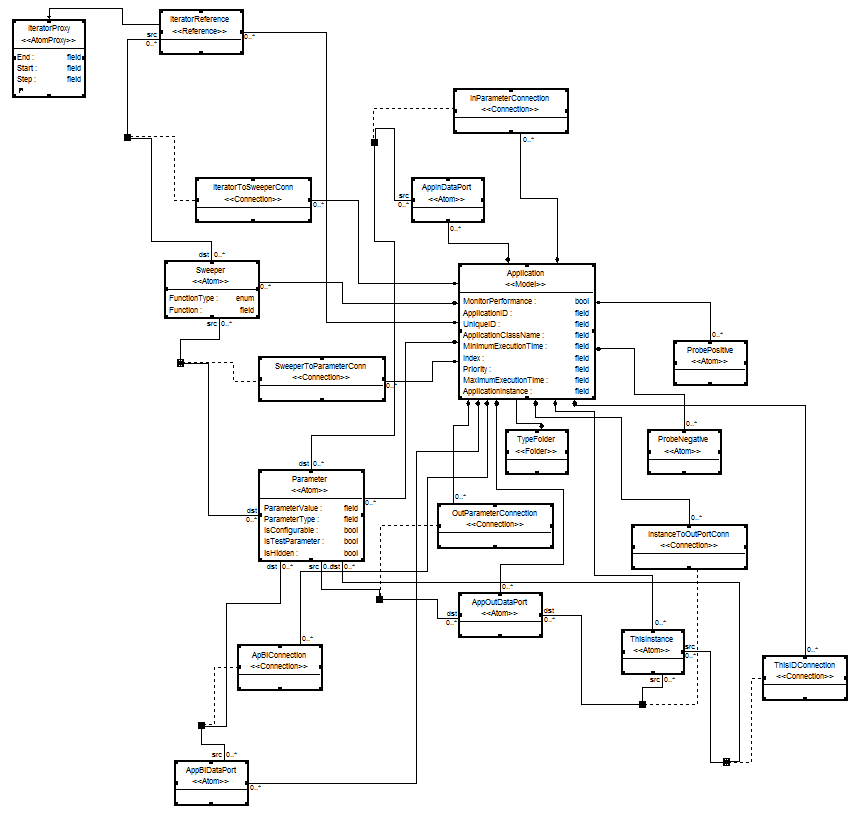
\includegraphics[width=0.60\textwidth]{figures/ApplicationMetaModel.png}
	\caption{Application metamodel in GME}
	\label{fig:ApplicationMetaModel}
\end{figure}

The Data Flow Aspect lays out the data ports that the application has and the parameters to configure the application. The data ports can be input only, output only and bidirectional. The application has the following attributes:

\begin{itemize}
	\item MonitorPerformance: Boolean flag to denote whether the performance of the application needs to be monitored
	\item ApplicationID: Unique identification number of application
	\item ApplicationClassName: Class name of the application's implementation
	\item MinimumExecutionTime: Minimum execution time of the application
	\item MaximumExecutionTime: Maximum execution time of the application
\end{itemize}

The parameters of the application have the following properties:

\begin{itemize}
	\item ParameterValue: Value of the application parameter
	\item ParameterType: Basic type of the application parameter (e.g. double, int)
	\item IsConfigurable: Boolean flag to denote if the parameter is a configurable parameter
	\item IsTestParameter: Boolean flag to denote if the parameter is a test parameter
\end{itemize}

The Test Definition Aspect provides Sweeper to vary the values of test parameters of an application and Negative Probe and Positive Probe to attach performance measurement points.

Sweeper is an important element in TSDML which has the following attributes:

\begin{itemize}
	\item Function Type: Internal function or look-up table. Internal function is a function of test series iterator whereas the look-up table may have specific values that an application can take.
	\item Function: The definition of the function.
\end{itemize}

Sweeper is attached to an application parameter and varies the value of the parameter based on the function provided in its attribute. A new value for an application parameter is used in each test case that will be generated from the model.

Figure \ref{fig:ApplicationModelDataFlow} shows the Data Flow and Figure \ref{fig:ApplicationModelTestSeries} shows the Test Series Definition aspect of sample application model.

\begin{figure}
	\centering
		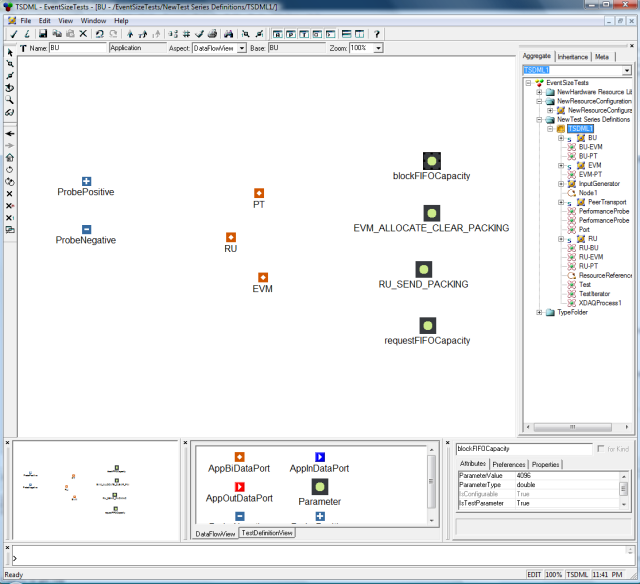
\includegraphics[width=0.60\textwidth]{figures/ApplicationModelDataFlow.png}
	\caption{Data Flow Aspect of a Sample Application Model}
	\label{fig:ApplicationModelDataFlow}
\end{figure}

\begin{figure}
	\centering
		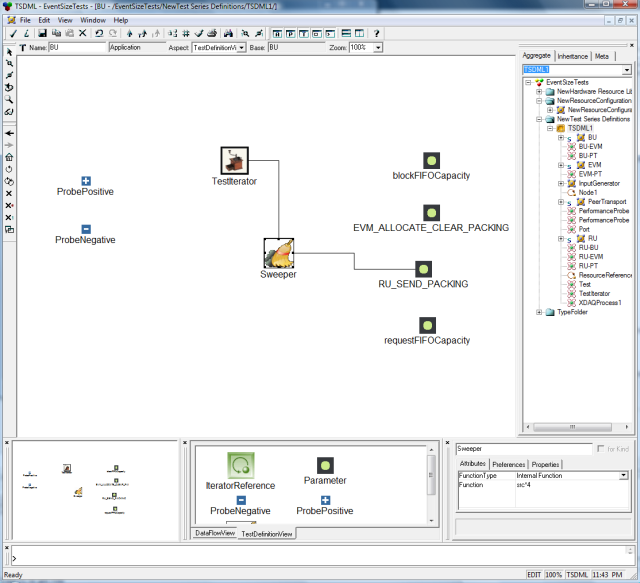
\includegraphics[width=0.60\textwidth]{figures/ApplicationModelTestSeries.png}
	\caption{Test Series Definition Aspect of a Sample Application Model}
	\label{fig:ApplicationModelTestSeries}
\end{figure}

Modeling application types in this manner tackles several challenges mentioned in the previous sections. This approach treats both the middleware and its applications as application types and enables modeling and configuration of them separately. For this reason, it will be possible to consider not only middleware-application relationships but also application-application relationships. In addition, it'll be possible to identify the couplings between middleware and applications that use its services.

****TODO: Change figures to metamodel figures. Will use the model figures in the implementation****

\subsubsection{Modeling Resources and Resource Configurations}
TSDML includes a way to model the resources to be used to deploy the system. A simple abstraction has been chosen for TSDML for modeling resources. However, it can easily be extended to drill down to the details of resources and resource management. Two main parts are the resource library and the resource configurations. TSDML has been constructed such that resource library collects models of the resources that can be used in a resource configuration. Resource configurations use references to resource models in the library to define specific configurations.

Resource is described as a \textit{Node} in TSDML. TSDML uses the following entities and their attributes to define a node:

\begin{itemize}
	\item Network Card (NIC)
	\subitem IP Address
	\subitem Network Type (e.g. Gigabit, Infiniband, etc.)
	\item Processor
	\subitem IP Address
\end{itemize}

\begin{figure}
	\centering
		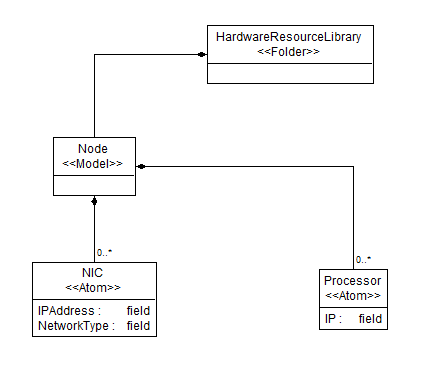
\includegraphics[width=0.60\textwidth]{figures/ResourceLibraryMeta.png}
	\caption{Resource Library Metamodel}
	\label{fig:ResourceLibraryMeta}
\end{figure}


Resource configuration model is described by a reference to a node that is created in the resource library model. The main point of a resource configuration model is to define the connections between the nodes. A connection between nodes is made through the \textit{Network} entity. TSDML uses the following entities and their attributes to define a resource configuration:

\begin{itemize}
	\item Node Reference: Reference to a node created in resource library
	\item Network
	\subitem Network Type (e.g. Gigabit, Infiniband, etc.)
\end{itemize}

\begin{figure}
	\centering
		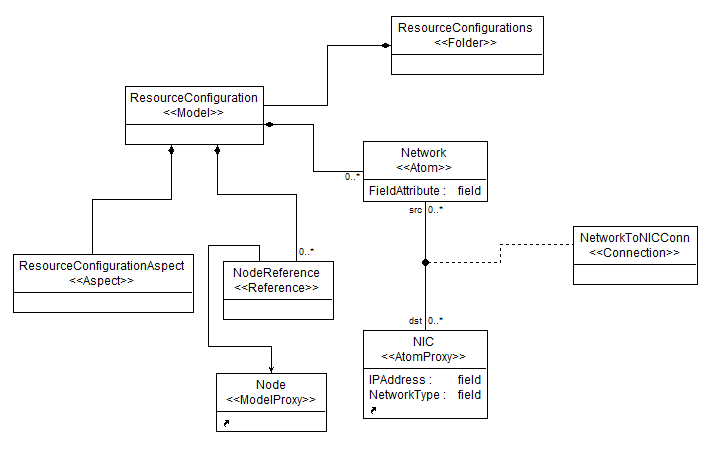
\includegraphics[width=0.60\textwidth]{figures/ResourceConfigMeta.png}
	\caption{Resource Configuration Metamodel}
	\label{fig:ResourceConfigMeta}
\end{figure}


\subsubsection{Parameterizing the Model}
\label{SubSubSection:Parameterizing}
As mentioned previously, it is desired that the TSDML model should be parametrized in order to be able to generate series of test cases from a single model. The parameterization is achieved by using ``Iterator'' and ``Replicator'' entities in the system model.

\textbf{Iterators} are used to define the series $i, j, k ...$ for the notions of $\left\{start, step, stop\right\}$. There can be many iterators in a test series definition.

\textbf{Replicators} are used to define the replication factor for the attached object. The replication factor determines how many of the object to which the replicator is attached to will be generated when the model is interpreted. Replicators are functions of iterators as in $r = K \times si$. There can be many replicators in a test series definition. Replicators must be attached to an iterator in the model since they are functions of iterators. They must also be attached to an application, network or context entity.

Figure \ref{fig:iterator-replicator} shows a possible example use of replicators and iterators in the model to generate multiple instances of two different application models. 

\begin{figure}
	\centering
		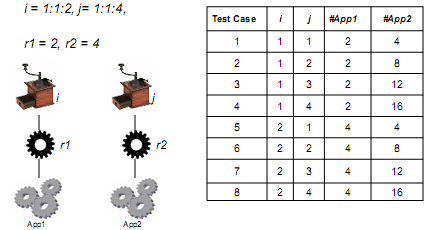
\includegraphics[width=0.90\textwidth]{figures/iterator-replicator.png}
	\caption{Use of iterators and replicators in the model}
	\label{fig:iterator-replicator}
\end{figure}

In the example, it is assumed that $i = 1:1:2$ and $j = 1:1:4$ and $r1 = 2$ and $r2=4$. By design, iterators function as the outer loop whereas the replicators function as inner loops. In this case, the table in Figure \ref{fig:iterator-replicator} shows the total number of test cases that will be generated and the numbers of App1 and App2 instances in those test cases. In this example, total of $8$ cases will be generated and number of App1 instances will change between $2$ and $4$ and the number of App2 instances will change between $4$ and $16$.

Iterators and connectors also function similarly when there is a connector between applications. Figure \ref{fig:iterator-connector} shows an example of such a situation. 

\begin{figure}
	\centering
		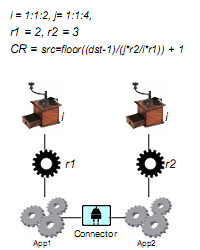
\includegraphics[width=0.40\textwidth]{figures/iterator-connector.png}
	\caption{Use of iterators and replicators with connectors}
	\label{fig:iterator-connector}
\end{figure}

\begin{figure}
	\centering
		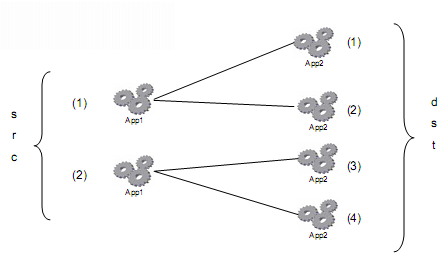
\includegraphics[width=0.80\textwidth]{figures/iterator-connector2.png}
	\caption{Resulting Configuration for Example 2}
	\label{fig:iterator-connector2}
\end{figure}

As described above, since connectors are boolean functions of iterators and replicators, it is possible to define the connection relation between applications with respect to the iterators and replicators to which the applications are attached to. In the example shown in Figure \ref{fig:iterator-connector}, iterator $i$ is defined as $i = 1:1:2$ and iterator $j$ is defined as $j = 1:1:4$ and replicators r1 and r2 are defined as $2$ and $3$ respectively. The connection relation between applications is defined as the boolean function $src = floor((dst-1)/(j \times r2 / i \times r1)) + 1$. As can be seen in the figure, App1 is the source (src) and App2 is the destination (dst). 

In order to fully understand what type of a model this example will lead to, we should first consider the iteration and replication of the applications. This example shares the same configuration for applications as shown in Figure \ref{iterator-replicator}. That is, there will be a total of 8 test cases. For the first test case, there will be 2 instances of App1 and 4 instances of App2. The connection between these applications is determined by the connection relation and results in the configuration shown in Figure \ref{iterator-connector2}. 

Modeling iterators and replicators as part of the TSDML aims to tackle the challenge of writing and managing many test configurations. By using iterators and replicators and taking advantage of auto generation capabilities of the modeling approach, a test engineer will be able to create and control many test cases with minimal effort. 

The concept of iterators and replicators easily and conveniently achieve the parameterization goal of the TSDML and enable creation of series of test cases from the single test template model. 

\subsubsection{Modeling Input Generator}
Input Generator is an important entity in the TSDML. It is not necessarily part of the overall system however it is crucial to model the input to the system for testing purposes.

In TSDML, input generator is modeled as a construct containing some parameters. The input generator is assumed to be used for generating events for the event based system. The following parameters make up the input generator:

\begin{itemize}
	\item Input Generator Parameter: Any parameter that may relate to modeling an input generator (e.g. mean, sigma, etc.)
	\item Random Distribution: Enumeration to model the type of distribution (e.g. Lognormal, normal, exponential, etc.)
	\item Parameter Sweeper: Similar to application types, a sweeper can be connected to parameters to vary the values of parameters for each test
	\item Iterator Reference: Reference to the iterator used for test series definition. 
\end{itemize}

Most important part of the input generator model is the parameter sweeper. It is the same sweeper that is used for varying values of application parameters. By connecting the iterator reference to a sweeper, values of input generator can be varied for each test case to be able to test the system against varying input data.

Based on the design of the system, the input generator can be connected to any application which accepts the input data and is the trigger for the operation of the system. Figure \ref{fig:InputGeneratorMetaModel} shows the Input Generator portion of the TSDML metamodel.

\begin{figure}[htb]
	\centering
		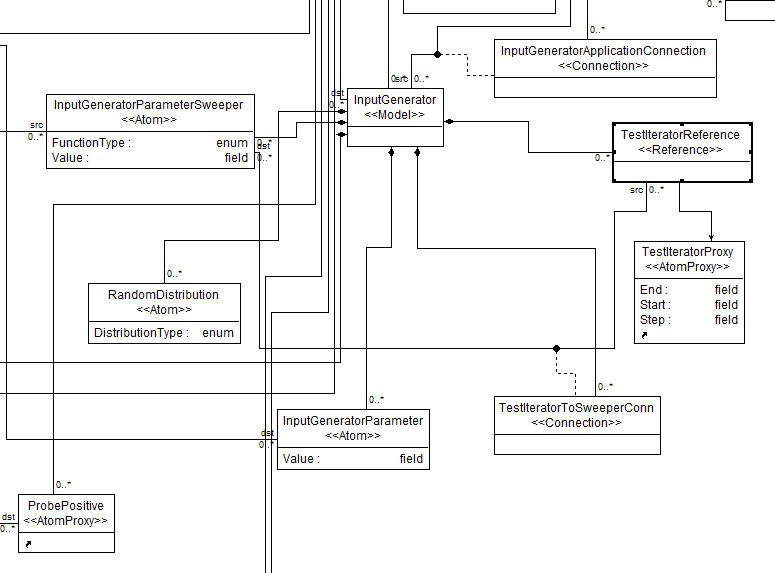
\includegraphics[width=0.70\textwidth]{figures/InputGeneratorMetaModel.PNG}
	\caption{Input Generator Meta Model}
	\label{fig:InputGeneratorMetaModel}
\end{figure}

\subsubsection{Modeling Test Series Definitions}

\begin{figure}[tbp]
	\centering
		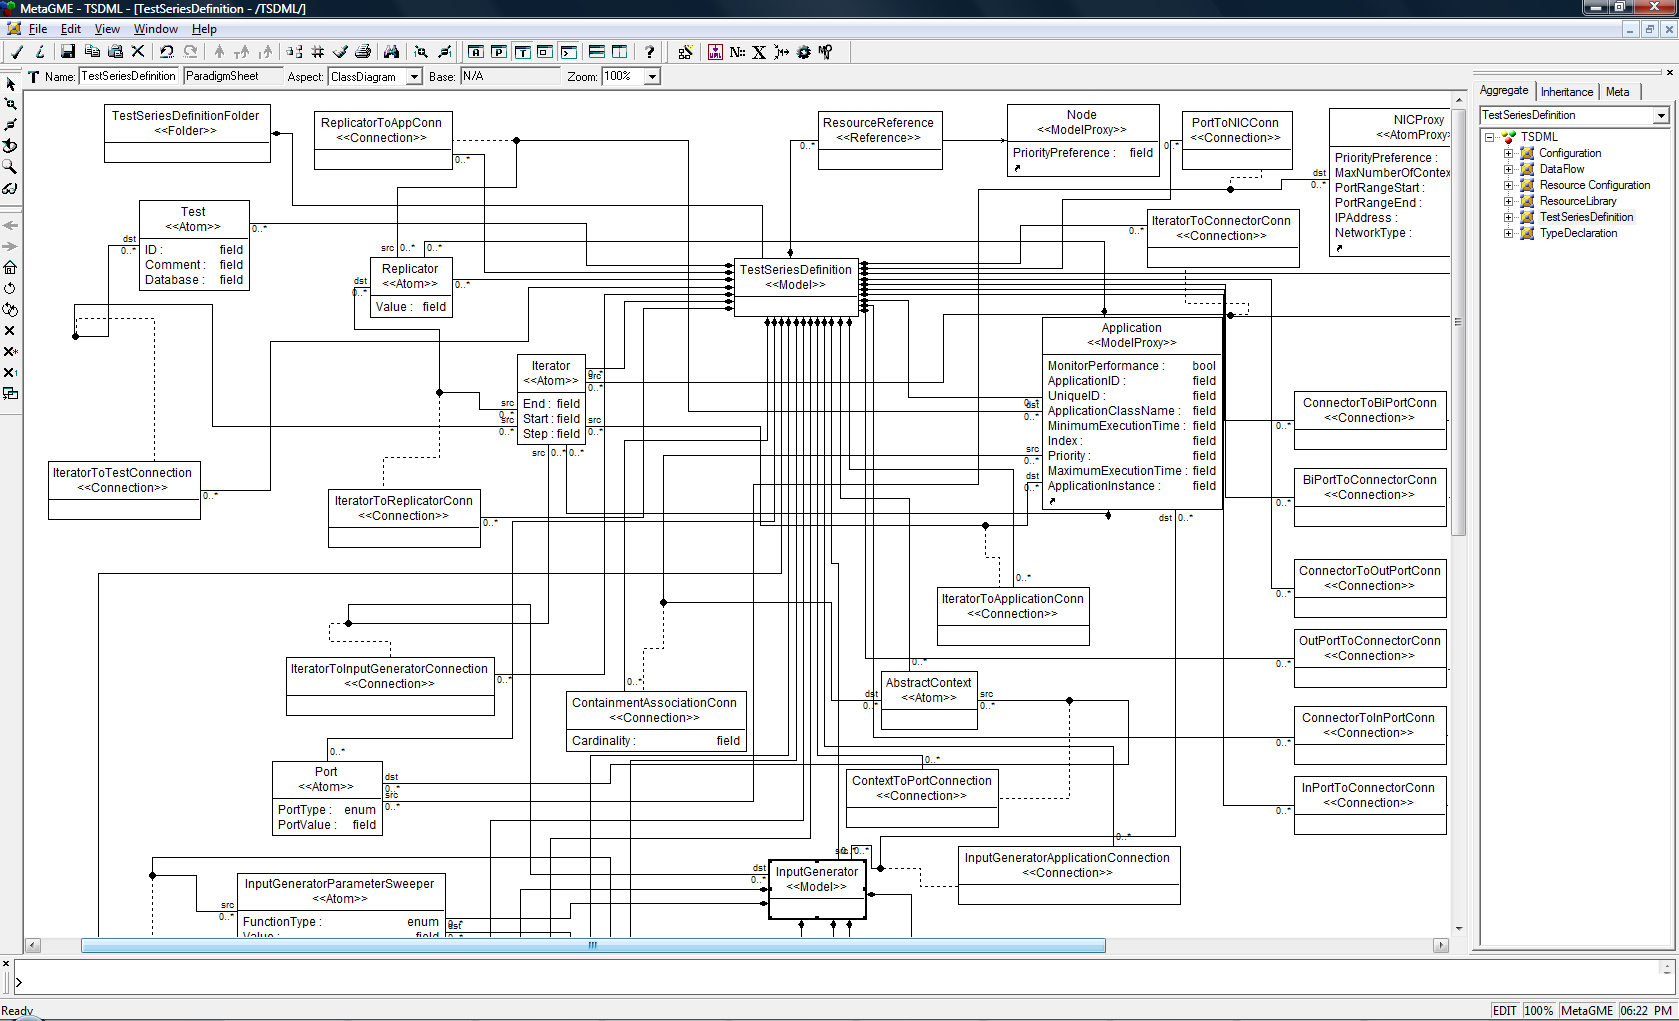
\includegraphics[width=0.90\textwidth]{figures/TestSeriesDefinition.png}
	\caption{Test Series Definition Meta Model}
	\label{fig:TestSeriesDefinition}
\end{figure}

Test series definition models bring together all the entities of the TSDML from a test generation perspective and enables generation of series of test cases utilizing model parametrization described in the previous subsection.

An important advantage of using MIC model based methodology is the ability to view the system to be modeled from different aspects and enable separation of design concerns. From this perspective TSDML defines three different aspects: Test Series Definition Aspect, Deployment Aspect, Performance Aspect. All there aspects of modeling a test series definition will be explained in detail.

The \textit{\textbf{Test Series Definition Aspect}} includes all the modeling elements that were described in the previous subsections. Test Series Definition aspect acts like a design surface for designing series of test cases. It contains the following modeling elements:

\begin{itemize}
	\item Application Reference
	\item Iterator
	\item Replicator
	\item Connector
	\item Input Generator
	\item Test entity
	\item Connections between these entities
\end{itemize}

References to application types and connectors that connect the applications make up the data flow among the applications. In order to create a test series definition not all application types need to be present. Different test series definitions with different applications and with same applications and different parameter values can be modeled since test series definitions are collected under a folder structure and lead to different set of test cases.

Iterators and replicators are the entities which define the scope of the series and add parameterization to the test series definition model. As described in "`Parameterizing the Model"', a replicator enables using a single application type and generate multiple application instances during test case generation. By use of replicators and iterators, it is possible to easily create a template of an application to be replicated at each step of test case generation.

Connector defines the relationship and data flow between the applications. When a connector entity is used to connect ports of two applications, it denotes that there is a data flow between those applications. As explained before, it is also a very powerful entity with its ConnectionRule property which is a function of the iterator. Making connections this way enables variations on the application structure that is to be tested.

The InputGenerator entity supplies the test data to the system to drive the test run. It can be connected to the applications which are expecting data to be enabled.

The Test entity is a placeholder entity which captures the general information about the test that is being designed. The information captured is used to store the results of the test run appropriately in a database or test log. The primary attributes of the Test entity are the Comment and Database fields. The Comment field is used to give a brief description of the test series being designed. The Database field is used to capture the name of the database that the test results will be saved to.

A test series definition is obtained when all these entities are connected to each other appropriately. The number of test cases that will be generated from one test series definition is based on the value of the iterator. 

The Test Series Definition aspect provides the solution for the challenge of manually creating several XML test configurations and makes the process easier to scale and less time consuming. In addition, by bringing together the pieces that are mentioned in the previous sections, this view makes it possible to span a considerable portion of the configuration space of parameter applications. This is made possible by being able to change application parameter values by means of Sweepers and control this change by iterators and replicators for each test case.

****TODO: May rewrite to better focus on answers to the challenges.****

The \textit{\textbf{Deployment Aspect}} includes modeling entities that can be used to devise different deployment scenarios for the system. The following entities can be used in this aspect:

\begin{itemize}
	\item Application (Reference)
	\item Resource (Reference)
	\item Middleware
	\item Port
\end{itemize}

Any common entities across aspects are carried over to the respective aspect. For this reason, the application reference is the same as the on used in the Test Series Definition aspect. The difference across different aspects is the perspective those entities are being looked at. While in the Test Series Definition aspect, the application reference was viewed from the perspective of creating a test series definition with multiple instances of applications generated automatically. In this aspect, the applications are viewed from a deployment perspective. The connections that are to and/or from an application reference are related to the deployment aspect of the system. 

Resource reference is a reference to any resource that is modeled in the Resources and Resource Configurations. Deployment aspect is the only place where a resource can be utilized because it's inherently related to deployment. From the testing perspective, having a resource model in this view makes it possible for a test designer to deploy a system on various resources and devise several test cases.

Another entity in the Deployment aspect is Middleware. It is a key entity for deployment because applications cannot run in absence of middleware and have to be deployed in a middleware instance. Technically, middleware is no different than an application, it's defined and modeled with application types. However, it's special in the sense that can contain other application types. As applications can be deployed on middleware, middleware is deployed on resources on specific ports.

Port, as the name suggests, is a logical entity used to define endpoint for the application on the resource that it is deployed to. It is used to connect middleware to a resource. Port has the following attributes:

\begin{itemize}
	\item Port Type: Type of port (e.g. TCP/IP, SOAP, etc.)
	\item Port Value: Value of port (e.g. 8080, 4000, etc.)
\end{itemize}

\textit{\textbf{The Performance Aspect}} includes entities related to capturing performance information about the system. The main entity of this aspect is the Performance Probe. It's designed to be analogous to a voltmeter or ammeter used to measure electric voltage and current in electronic circuits. In this manner, a performance probe is connected to positive and negative end points and measures a performance metric between those points.

A performance probe has one attribute:
\begin{itemize}
	\item Metric: It's an enumeration of possible performance metrics to be measured (e.g. throughput, latency, bandwidth).
\end{itemize}

For example, when a performance probe is connected between the negative probe end of App1 and positive probe end of App2 and its metric is set as Throughput, it means that throughput between App2 and App1 will be measured.

All the aspects of the Test Series Definition make up the main parts of the TSDML. Test series definition uses the modeling constructs defined elsewhere to model a system from test, deployment and performance points of views. 

\subsection{Modeling Behavior with DEVS}
The Test Series Definition Modeling Language makes it possible to model the system from various perspectives. It is a graphical domain specific language that can be used to capture structure and data flow of a system from a higher level of abstraction. TSDML also enables the design of a system from the testing perspective. 

In model driven engineering, the crucial step after modeling a component or a system is to be able to interpret the meaning of the abstractions in the model. The artifact of such interpretation can be a design document, source code, etc. In the case of the approach described in this chapter and the TSDML, the desired artifact is several test cases (e.g. in the form of XML configurations) that can be executed on the real implemented system. 

In some cases, the real implementation of the system modeled by TSDML may not be available. Moreover, it may not always be feasible to execute the test cases on the real system. An implementation of the system may not yet be available or it may be costly to run unpredictable tests on the real implementation or replicate the real system setup for testing purposes. In such cases, it is important to be able to model the behavior of the system as well. 

In the approach described in this chapter, the behavior model of the applications of the system is created using the Open DEVS modeling formalism. A background on Open DEVS is given in Chapter \ref{Chapter:DEVS}. 

DEVS modeling formalism and the underlying simulation framework enables the execution of test cases generated from TSDML on a simulated system. In order to achieve that, each application type that is modeled using TSDML should have a corresponding DEVS behavior model. An application is modeled using DEVS as described in Chapter \ref{Chapter:DEVS}. The main aspect of this process is correctly determining:

\begin{itemize}
	\item States of the application
	\item Input and output events of the application
	\item Input and output connections/ports of the application
\end{itemize}

Since DEVS is an event based framework, it is possible model the data flow and interactions among applications. In a middleware based system, it is particularly important to determine interactions between applications. It is possible with DEVS to model the application interaction in such a way that no application can talk to each other without going through middleware. 

An example implementation of a DEVS model will be given in Chapter \ref{Chapter:Implementation}.

\section{Closing the Loop: Performance Engineering}
Size and complexity of software systems are increasing and there is increasing demand for component based distributed applications and systems. Performance characteristics such as throughput and scalability are crucial quality attributes of such systems. For this reason, it is very critical to validate that the system satisfies the performance requirements. Performance testing is a way to evaluate performance characteristics. 

IEEE Standard Glossary of Software Engineering Terminology defines performance testing as ``testing conducted to evaluate the compliance of a system or component with specified performance requirements'' \cite{ieee_90}. In \cite{Weyuker00}, Weyuker and Volokos list possible goals for performance testing as follows:
	
\begin{enumerate}
	\item ``the design of test case selection or generation strategies specifically intended to test for performance criteria rather than functional correctness criteria.''
	\item ``the definition of metrics to assess the comprehensiveness of a performance test case selection algorithm relative to a given program.''
	\item ``the definition of metrics to compare the effectiveness of different performance testing strategies relative to a given program.''
	\item ``the definition of relations to compare the relative effectiveness of different performance testing strategies in general.''
	\item ``the comparison of different hardware platforms or architectures for a given application.''
\end{enumerate}

The scope of the approach described here lies within the boundaries of the definition and the first of the goals given above. Although the description and the goal is pretty clear and easy to understand, some questions and details are hidden below the surface. Non-functional requirements of a system define how the system is to operate whereas functional requirements define how the system should behave. Non-functional requirements are harder to gather and define than functional requirements. Similar difficulty exists in testing non-functional requirements \cite{Chu99}. The difficulty generally stems from the nature of non-functional requirements being observed and evaluated subjectively. 

Performance is such a non-functional system requirement. Although it can be measured, it is still subjective. Non-functional requirements like performance are usually evaluated, analyzed or even predicted during design time rather then tested during run-time. 

\begin{figure}
	\centering
		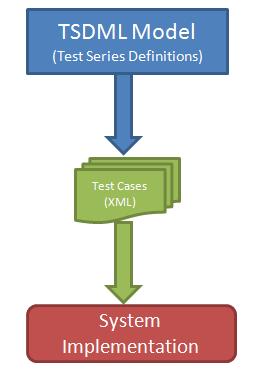
\includegraphics[width=0.35\textwidth]{figures/SystemRun.png}
	\caption{Test Cases Run on System Implementation}
	\label{fig:SystemRun}
\end{figure}


In the previous sections, an approach for modeling a system's behavior and structure from performance perspective was described. The approach described enabled generation of many test cases from TSDML models to be executed on a DEVS simulation engine running behavioral models of the system. There are two paths that can be taken from the model level to the system level:

\begin{itemize}
	\item Test cases may be executed on the real system (\ref{fig:SystemRun}). Running test cases on the real system for performance testing potentially gives the best results. However, this option may not always be available since it may be costly to run test cases with unpredictable outcomes on a real system. In such a case, it may be desirable to replicate the real system in a similar environment which may also be a costly operation. 
	\item Test cases may be executed on a simulation environment using behavioral models for the applications (\ref{fig:SimulationRun}). This path is less costly albeit the quality of performance test results are highly dependent on the quality of the system behavioral models.
\end{itemize}

\begin{figure}
	\centering
		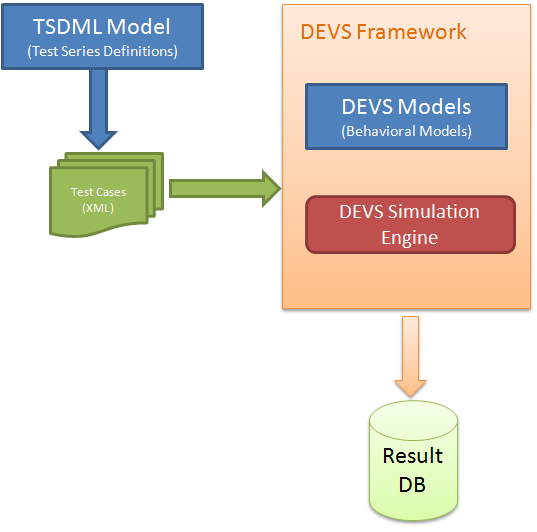
\includegraphics[width=0.40\textwidth]{figures/SimulationRun.png}
	\caption{Test Cases Run on Simulation Engine}
	\label{fig:SimulationRun}
\end{figure}

In either case mentioned above, there needs to be a way to make an assessment about the results of the test run. If performance requirements were clearly captured and each performance metric could be measured at the end of a test run, it might be possible to make pass/fail decision on the test run. However, the question is: is it desirable to merely verify performance, or in general non-functional requirements, in the same manner as functional requirements? One may argue that non-functional requirements testing phase in the development life cycle is more about observing, understanding how the system performs in different conditions, environments or with different system parameters. It is more valuable to be able to analyze test run results, reason about the system performance, and identify relationship of system parameters with performance then to make a pass/fail decision. From this perspective, (performance) testing approaches (performance) engineering. In this sense, it is crucial to be able to feed the results of a test run back into the system, thus closing the loop. This does not necessarily mean to automatically feed a test run result back into the system. This feedback may be in the form of understanding more about the system and devising more and interesting test cases with variations in system parameters or system environment. 

It is important to note that there is extensive literature on performance prediction from performance models and those literature was investigated in \cite{areapaper}. However, the approach described here is not about predicting the performance of a system from performance models as outline above. It is important to make the distinction between creating a performance model for a system and creating a system model and including a  performance aspect. In the approach described here, in a typical model based development sense, behavioral and structural abstractions of a system are captured in a system model and this model is extended from performance point of view. Since it is also possible to generate series of test cases from this system model, it is possible to run the actual test cases either on the real system or in a simulation environment to reason about the actual performance of the system.

\subsection{Performance Monitoring}
****TODO****

\subsection{Perturbation and Sensitivity Analysis}
Perturbation and sensitivity analysis methods that can be used to analyze results of a performance run. Using these techniques, one can observe the output of a system

-running the tests on the actual system automatically closes the loop
-performance engineering will give an idea about how the system performs
-not interested in prediction
-interested in what parameter change in the system cause what performance implication
-so far described test generation and execution. if tests run on real system, monitoring system performance will give information about the performance of the system. if tests run on simulation (in our case), need to measure and analyze the results to feed the findings back into the system. 
-design time performance analysis after simulation
-may reference from Prof. Karsai's monitoring book. Talk about monitoring but say we are interested in performance engineering.


\section{Summary}
****TODO****
	\chapter{Background on DEVS Modeling Formalism}
\label{Chapter:DEVS}

Discrete Event System Specification (DEVS) is a modeling and analysis formalism for discrete event systems \cite{Zeigler84}. Modular and hierarchical moduling views are two important aspects in DEVS formalism. Modularity is achieved by input and output events whereas hierarchical aspect is realized by the coupling operation.

A DEVS system is formed of states, input and output events, a notion of time, and functions that describe how the system evolves with respect to input and output events.

There are two types of DEVS models. Atomic DEVS models enable a system to be modeled modularly by first creating models by simple fundamental dynamic behaviors. Coupled DEVS models enables the definition of the system hierarchically by coupling the atomic models to create a complete system specification. Mathematical definitions of those models will be given in the next sections.

\section{Atomic DEVS Models}

\begin{figure}
 \centering
 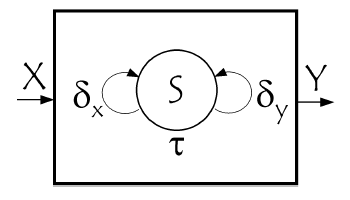
\includegraphics[width=0.75\textwidth]{figures/atomicdevs.png}
 % atomicdevs.png: 143406760x143406768 pixel, 0dpi, infxinf cm, bb=
 \caption{Symmetric Structure of Atomic DEVS}
 \label{fig:atomicdevs}
\end{figure}

An atomic DEVS is a 7-tuple structure $A = < X, Y, S, s_{0}, \tau, \delta_{x}, \delta{y} >$ \cite{Devspp} where

\begin{itemize}
 \item $X$ is a set of \textit{input events}.
 \item $Y$ is a set of \textit{output events}.
 \item $S$ is a set of \textit{states}.
 \item $s_{0} \in S$ is the initial state.
 \item $\tau ; S \rightarrow T$ is the \textit{time advance function} where $T = [0,\infty]$ is the set of non-negative real numbers plus the transfinite number, infinity. This function is used to determine the lifespan of a state.
 \item $\delta_{x} : P \times X \rightarrow S \times {0,1}$ is the \textit{input transition function} where $P = \left\{(s, t_{s}, t_{e}) | s \in S, t_{s} \in T, t_{e} \ in [0, t_{s}]\right\}$
\end{itemize}

There are two types of transitions in an atomic DEVS model: external and internal transitions. These transitions are the only ways a model can change its state. Internal transitions are time-based. That is, a transition occurs when the elapsed time reaches to the lifetime of the state which is defined by $\tau(s)$. An internal transition not only causes a state change but may also generate an output event. External transitions are event-based. That is, a transition occurs when an input event arrives. An input event causes a state change when the conditions given by $\delta_{x}$ is satisfied. External transitions are instantaneous and only trigger state change and do not generate an output event.

Figure \ref{fig:atomicdevs} demonstrates an atomic DEVS model. 


\section{Coupled DEVS Models}

A coupled DEVS is also a 7-tuple structure \cite{Devspp} $N = < X, Y, D, \left\{M_{i}\right\}, EIC, ITC, EOC >$ where

\begin{itemize}
 \item $X$ is a set of input events
 \item $Y$ is a set of output events
 \item $D$ is a set of names of subcomponents
 \item $\left\{M_{i}\right\}$ is a set of DEVS models where $i \in D$. $M_{i}$ can be either atomic DEVS model or a coupled DEVS model
 \item $EIC \subseteq X \times \underset{i \in D}{\cup} X_{i}$ is a set of external input couplings where $X_{i}$ is the set of input events of $M{i}$.
 \item $ITC \subseteq \underset{i \in D}{\cup}Y_{i} \times \underset{i \in D}{\cup} X_{i}$ is a set of internal couplings where $Y_{i}$ is the set of output events of $M_{i}$.
 \item $EOC \subseteq \underset{i \in D}{\cup}Y_{i} \times Y$ is a set of external couplings.
\end{itemize}

A coupled DEVS model defines the subsystems that are contained by the model and how there are connected to each other. Coupled DEVS models realize the modular and hierarchical aspect of the DEVS formalism by enabling a system designer to build a larger system by designing and connecting simpler subsystems. Although it is not impossible to create a complete system only with atomic models, it is very tedious and error prone. Coupled DEVS model eliminates this complexity and lets subsystems be composed together and connected to each other enabling a better system specification.

Since the resulting DEVS model is modular and hierarchical, events generated within a subsystems can propoage through other parts of the subsystem horizantally, or through other subsystems vertically within the hieararchy of the system through well defined interfaces. 

\section{Summary}

DEVS formalism  provides the means to describe discrete event systems and provides constructs like time, events, states and transitions as well as composition of models. In this research, DEVS was chosen to be used to model parts of a distributed data acquistion system. Event-based nature of the data acquistion system made DEVS the proper tool to model its middleware and applications using the DEVS modeling formalism. Open DEVS simulation framework \cite{Devspp} provides suitable ground work to model applications as DEVS models and simulate the complete system.
	
	\chapter{Background on CMS DAQ System}
\label{Chapter:DAQ}
The Compact Muon Solenoid (CMS) experiment is a particle physics detector built on the proton-proton Large Hedron Collider (LHC) being built at CERN in Switzerland. CMS aims to to explore physics at the electron volt and to discover the Higgs boson. CMS is designed as a general-purpose detector and is going to be capable of studying results of proton collusions to take place inside the LHC. 

An experiment at a hadron collider requires a sophisticated trigger and data acquisition (DAQ) system because of very high collision and overall data rates. The frequency of protons crossing each other at the LHC is 40 MHz \cite{CMSTDR}.

The main goal of the CMS Trigger and Data Acquisition System (TriDAS) is to inspect the detector information at 40 MHz frequency and to select events and to store for offline processing. The events are selected at the maximum rate of $O(10_{2})$. There are two steps in the functionality of the system. The first step, which is called the Level-1 Trigger \cite{CMSTDR}, is designed to reduce the rate of events selected for offline processing to less than 100 kHz. The second step, which is called High-Level Trigger (HLT), is designed to further reduce the 100 kHz. of the Level-1 Trigger to the final output rate of 100 Hz. 

Functionality of the CMS DAQ and HLT is given in the CMS DAQ Technical Design Report as follows \cite{CMSTDR}:

\begin{itemize}
	\item ``perform the readout of the front-end electronics after a Level-1 Trigger accept''
	\item ``execute physics selection algorithms on the events read out, in order to accept the ones with the most interesting physics content''
	\item ``forward these accepted events, as well as a small sample of rejected events, to the online services which monitor the performance of the CMS detector and also provide the means of archiving the events in mass storage''
\end{itemize}

Figure \ref{fig:triggerdaq} shows the data flow in the Trigger/DAQ system and also visualizes the Level-1 Trigger and HLT stages mentioned above.

\begin{figure}
	\centering
		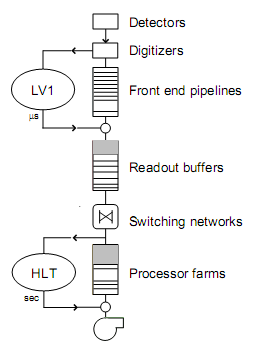
\includegraphics[width=0.45\textwidth]{figures/triggerdaq.png}
	\caption{Data Flow in the Trigger/DAQ System}
	\label{fig:triggerdaq}
\end{figure}

\section{DAQ Architecture}
Figure \ref{fig:xdaqarch} shows the architecture of the CMS DAQ system. The system consists of the following elements:

\begin{itemize}
	\item \textbf{Detector Front-ends} are the components that are connected to the front-end electronics to store the data from them as the Level-1 Trigger accept signal is received. 
	\item \textbf{Readout Systems} are the components that are connected to the Front-End System (FES) to read the data from the detector. Readout systems store the data until they are sent to the processor to which will analyze the event.There are about 500 components which are called ``Readout Columns''. Each Readout Column consists of a number of Front-End Drivers (FEDs) and one Readout Unit (RU). RU is responsible for keeping the event data in its buffer and interfacing to the switch.
	\item \textbf{Builder Network} is a collection of networks providing the interconnections between the Readout and Filter Systems. It can handle 800Bg/s sustained throughput to the Filter Systems.
	\item \textbf{Filter Systems} are the processors that the RUs provide the events with. Filter systems are the entities that decide whether a supplied event is interesting and will be kept for offline processing or not. The interestingness of an event is determined by executing the High-Level Trigger algorithms. There are about 500 entities which are called ``Filter Columns''. Each of those include one Builder Unit (BU). A BU is responsible for receiving incoming data fragments that correspond to a single event and building them into full event buffers. 
	\item \textbf{Event Manager} controls the flow of events in the system. Event Manager (EVM) serves as a centralized intelligence of event management.
	\item \textbf{Computing Services} are composed of all the processors and networks that receive filtered events and some of the rejected events from the Filter Farms.
	\item \textbf{Controls} are responsible for the user interface and the configuration and monitoring of the DAQ.
\end{itemize}

\begin{figure}
	\centering
		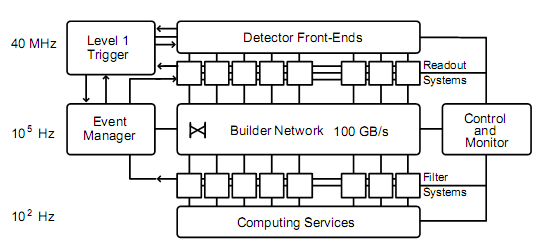
\includegraphics[width=0.90\textwidth]{figures/xdaqarch.png}
	\caption{CMS DAQ System Architecture}
	\label{fig:xdaqarch}
\end{figure}

Given the component breakdown of the system it is possible to identify four stages of system functionally. First stage is a detector readout stage where events are collected and stored in buffers. The second stage is the event building stage, where all data corresponding to a single event are collected from the buffers. The third stage is the selection stage where High-Level Trigger in the processor processes the event. The final stage is the analysis and storage stage where the events that are selected in the previous stage are sent to the Computing Services for additional processing for storage or further analysis. 

XDAQ uses a format called I20 data binary data format. I2O (Intelligent Input Output) is an I/O architecture specification developed by a consortium of computer companies called the I2O special Interest Group (SIG) for managing devices. The details of the I2O message format is not in the scope of this research. However, more information about the details of the I2O specification may be obtained from \cite{I2O}.


\section{Event Builder}
The main task of the DAQ system is to read each event's corresponding data out of the FEDs and merge it into the single structure called ``physics event'' and to transmit the physics event to a filter farm consisting of processor that execute physics algorithms that decide whether the event should be kept for further processing or discarded \cite{CMSTDR}. The Event Builder (EVB) is the central component of the DAQ system and includes the components that are responsible for this task.

Figure \ref{fig:builder} shows a more detailed version of the DAQ architecture depicted in Figure \ref{fig:xdaqarch}.

\begin{figure}
	\centering
		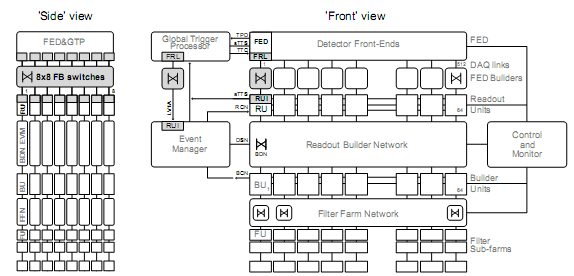
\includegraphics[width=0.90\textwidth]{figures/builder.png}
	\caption{Front and Side Views of the DAQ}
	\label{fig:builder}
\end{figure}

In the first of the stages that were idenfied above, there exist 8 FEDs that the RUs read data from and perform merging of event data fragments into larger data blocks called ``super-fragments'' or ``s-fragments''. This arrangement makes up a 64 ``FED Builders'' each of which consists of 8 FEDs, a 8x8 switch, and 8 RUs. Readout data is distributed among 64 RUs to maximize readout bandwidth. Thus, parts of data from a single event are buffered in 64 RUs. In the second state, 64 BUs which read out the data from a single event contained in 64 RUs and build these 64 s-fragments to form a single event. RUs and BUs are connected to each other through a 64x64 switch. The group of 64 RUs, the 64x64 switch and 64 BUs are called the ``RU Builder''. The full XDAQ system is composed of 64 FED Builders and 8 RU Builders. Figure \ref{fig:3dxdaq} shows the three-dimensional representation of the system \cite{CMSTDR}.

\begin{figure}
	\centering
		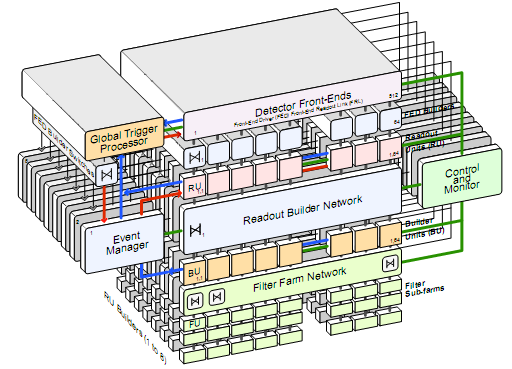
\includegraphics[width=0.90\textwidth]{figures/3dxdaq.png}
	\caption{Three-Dimensional View of the System}
	\label{fig:3dxdaq}
\end{figure}



\section{RU Builder}

This research is mainly interested in the components of the RU Builder as the experimental platform. Figure \ref{fig:evbsystem} shows the event builder and how the RU Builder is connected to the rest of the system \cite{rubuilder}. 

RU Builder consists of several applications. There is a single Event Manager (EVM), one or more readout units (RUs), and one or more builder units (BUs). The trigger adapters (TAs), readout unit inputs (RUIs) and filter units (FUs) are external to the RU Builder and are not in the scope of the experimental platform of this research. 

\subsection{Event Manager (EVM)}
EVM is the application that controls the flow of event data through the RU Builder. Figure \ref{fig:evm} shows the internal FIFOs of the EVM and its dynamic behavior.

In the first step, EVM receives trigger data of an event from the RUI. In step 2, EVM assigns a free event ID to the trigger data. In step 3, EVM requests the RUs to readout the event's data. In step 4, BU asks the EVM to allocate it an event. In this request, BU may also send an event ID to be cleared. In step 5, EVM saves the event ID received from BU as a free ID. In step 6, EVM sends the BU a confirmation of the allocation by sending the requesting BU the assigned event ID and trigger data of the allocated event. \cite{rubuilder}

\begin{figure}
	\centering
		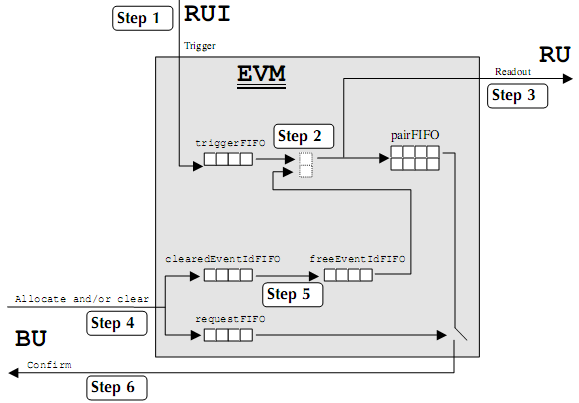
\includegraphics[width=0.90\textwidth]{figures/evm.png}
	\caption{Dynamic Behavior of EVM}
	\label{fig:evm}
\end{figure}

\subsection{Readout Unit (RU)}
RU is the application that buffers the s-fragments until there is a BU request. Figure \ref{fig:ru} shows the internal FIFOs of the RU and its dynamic behavior.

\begin{figure}
	\centering
		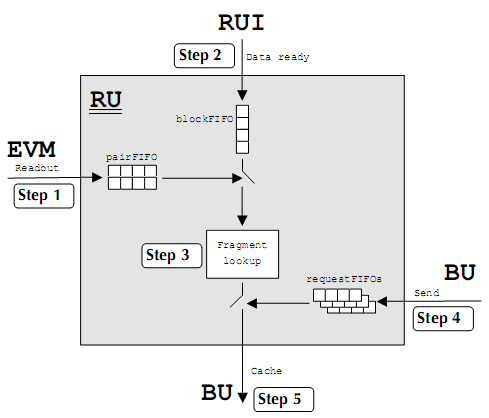
\includegraphics[width=0.90\textwidth]{figures/ru.png}
	\caption{Dynamic Behavior of RU}
	\label{fig:ru}
\end{figure}

In the first step, RU receives a pair of ``event ID/trigger event number'' and asks the RU to readout the data of the assigned event ID. In step 2, RUI tells the RU that event's data is ready to for readout and processing. In step 3, a RU fills in its fragment lookup table with each s-fragment for which it received pair for from the EVM. In step 4, BUs request from RUs the s-fragments of the events that they received confirmation for from the EVM. In step 5, a RU fulfills the request from a BU with s-fragments retrieved from the s-fragment from its fragment lookup table and asks the BU to cache the events data \cite{rubuilder}.

\subsection{Builder Unit (BU)}

BU is the application that is responsible for event building. Figure \ref{fig:bu} shows the internal FIFOs of the RU and its dynamic behavior.

\begin{figure}
	\centering
		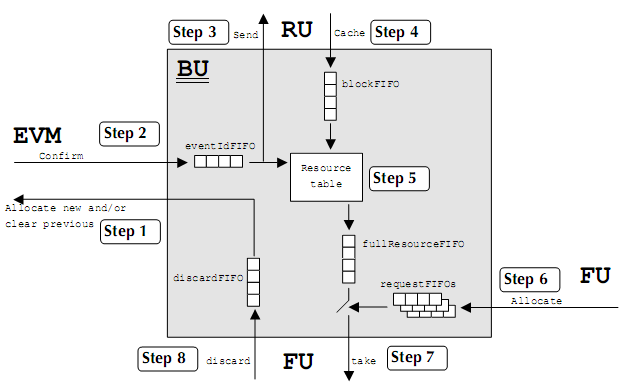
\includegraphics[width=0.90\textwidth]{figures/bu.png}
	\caption{Dynamic Behavior of BU}
	\label{fig:bu}
\end{figure}

In the first step, the BU with free capacity asks the EVM to allocate it an event. In step 2, BU receives the confirmation of event allocation from the EVM along with the event ID and trigger data of an event which makes up the first s-fragment of the event. In step 3, the BU asks the RUs for the rest of the event's s-fragments. In step 4, the BU receives the the rest of the event's s-fragments from RUs, and caches them in its block FIFO. In step 5, the BU builds the event's s-fragments into one whole event in its resource table. In step 6, FUs requests an event from BU for processing. In step 7, BU allocates a whole event to the requesting FUs. In step 8, when a FU finishes processing an event, it asks BU to discard the event ID corresponding to processed event \cite{rubuilder}.

\section{Summary}
CMS DAQ system is the data acquisition system for the CMS experiment. In this chapter, basic information about the architecture of the CMS DAQ system was given. The focus was given on the Event Builder and more specifically the RU Builder and its applications. RU Builder applications are used as part of the experimental platform for this research. 
	\chapter{Model Based Performance Engineering of CMS DAQ System}
\label{Chapter:Implementation}

In the previous chapters the methodology of the approach was described along with information on TSDML and DEVS modeling formalism. A background information about the CMS DAQ system was also given in Chapter \ref{Chapter:DAQ}. In this chapter, details of the implementation of the approach on the CMS DAQ system will be explained. 

The first section focuses and its subsections focus on describing the system under test and how it's broken into layers. The next section describes in detail how the applications in the system are modeled in DEVS modeling formalism. The third section talks about the performance aspect captured in the models. The fourth section explains the implementation of the random input data generator used to feed data into the simulation system. The next section lays out the communication interfaces between applications. Section five describes how the system is modeled in TSDML for test generation. Sections six and seven focus mainly on performance engineering and analysis of experiment results.   

\section{System Under Test}
The system that is modeled for performance testing/engineering is a middleware based distributed system which can be depicted in three layers as shown in Figure\ref{fig:systemfigure}.

\begin{figure}
 \centering
 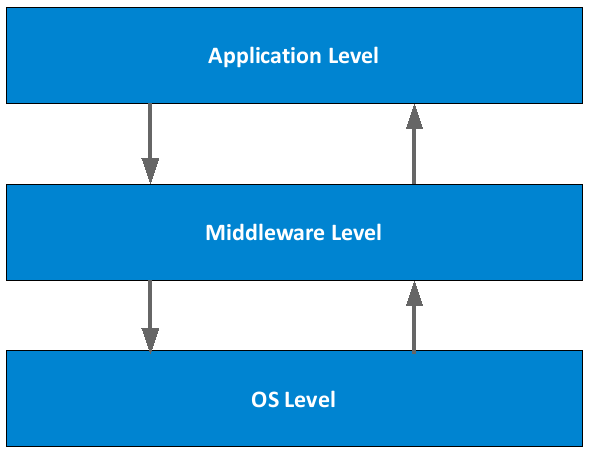
\includegraphics[width=0.6\textwidth]{figures/SystemFigure.png}
 % SystemFigure.png: 1179666x1179666 pixel, 0dpi, infxinf cm, bb=
 \caption{System Architecture}
 \label{fig:systemfigure}
\end{figure}

The modeled system is based on the XDAQ framework which is developed at CERN as a platform for the development of distributed data acquisition system \cite{CMSTDR}. A brief background on CMS XDAQ system is given in Chapter \ref{Chapter:DAQ}

In the upcoming sections, implementation of components of the system under test will be described. A depiction of the system under test as implemented can be seen in Figure \ref{fig:SUT}.

\begin{figure}
	\centering
		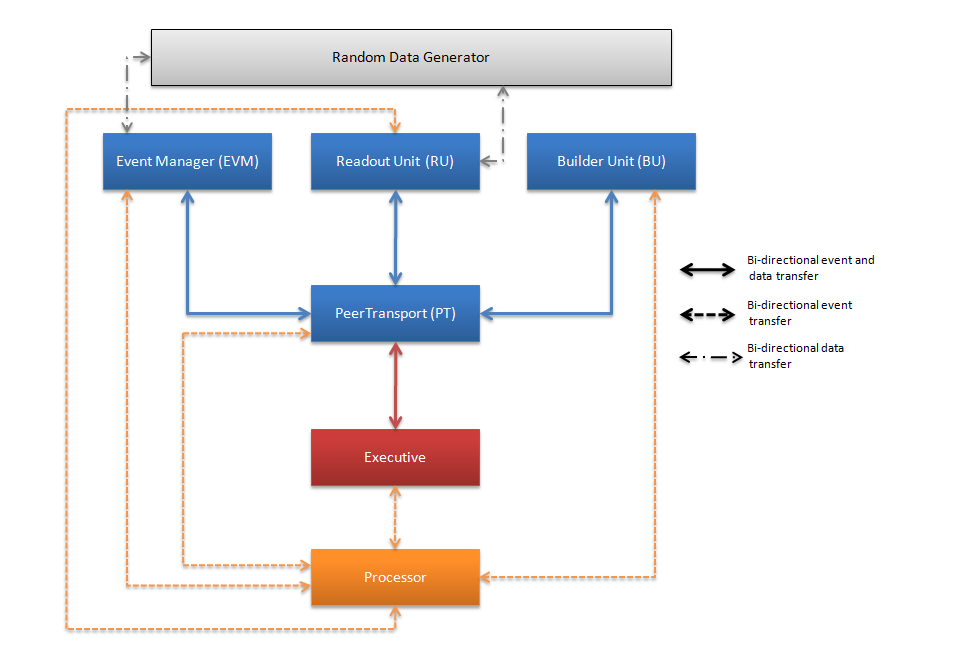
\includegraphics[width=0.90\textwidth]{figures/SUT.png}
	\caption{Implementation of System Under Test}
	\label{fig:SUT}
\end{figure}

\subsection{Application Layer}
There are four applications that exist in the application level. Those are Event Manager (EVM), Readout Unit (RU), Builder Unit (BU), and Peer Transport (PT).


Peer Transports are special applications that carry out the data transmission in the distributed programming environment. Data transmission in XDAQ and Peer Transports are explained in detail in the CMS DAQ Technical Design Report \cite{CMSTDR}. 

EVM, RU and BU applications form the RU Builder which is part of a larger system called the event builder (EVB). Given the distributed nature of the EVB, it is responsible with reading event fragments from one set of nodes and assembling them into entire events on another set of nodes. Figure \ref{fig:evbsystem} shows the event builder and how the RU Builder is connected to the rest of the system \cite{ru}. 

\begin{figure}
	\centering
		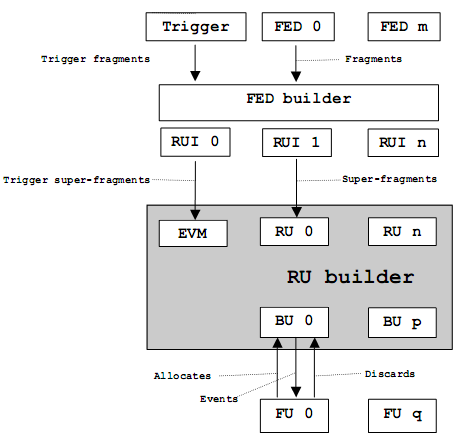
\includegraphics[width=0.90\textwidth]{figures/evbsystem.png}
	\caption{RU Builder Connected to Event Builder}
	\label{fig:evbsystem}
\end{figure}

This research is interested in the RU Builder and the applications that make up the RU Builder. Details of all the other components are given in \cite{CMSTDR}.

Event Manager (EVM) is the component which is responsible for determining the data flow in the RU Builder. Mainly, EVM assigns event id's to the events coming into the RU Builder. In addition, EVM manages the lifetime of the event id's as long as they are in the RU Builder. For this reason, EVM is the only component that knows about the status of the assigned event id's being processed in the RU Builder. EVM is in communication with all the RUs and BUs in the RU Builder \cite{CMSTDR}.

Readout Unit (RU) is the component which is responsible for reading super-fragments, keeps them in the memory until there is a request from the Builder Unit, and transmits the requested super-fragments as a response to the request \cite{CMSTDR}. 

Builder Unit (BU) is the component which is responsible for building complete events from the super-fragments that are in RUs. As BU builds complete super-fragments, it keeps them in its buffer until they are requested by the Filter Unit. Filter Unit is the computational unit of the Filter Farm which runs the physics algorithms \cite{CMSTDR}.

\subsection{Middleware Layer}
In the XDAQ architecture, the middleware layer is called the Executive Framework which is basically a XDAQ application called Executive. In a distributed manner, a copy of the Executive is run on every node that participates in data acquisition and event building. 

In the next section, how these application components are modeled in the context of Open DEVS framework will be explained.

\section{Application Simulation Models}

\subsubsection{Event Manager (EVM)}
EVM is responsible for controlling the flow of event data in the system. In the meantime, the EVM assigns event id's to the events that are generated. For the purposes of simulation, dummy event data is generated by the component called InputGenerator. Details of the InputGenerator will be explained later.

Figure \ref{fig:evm_behavior} shows the dynamic behavior of the EVM and the input/output events that it exchanges with the other applications.

\begin{figure}
	\centering
		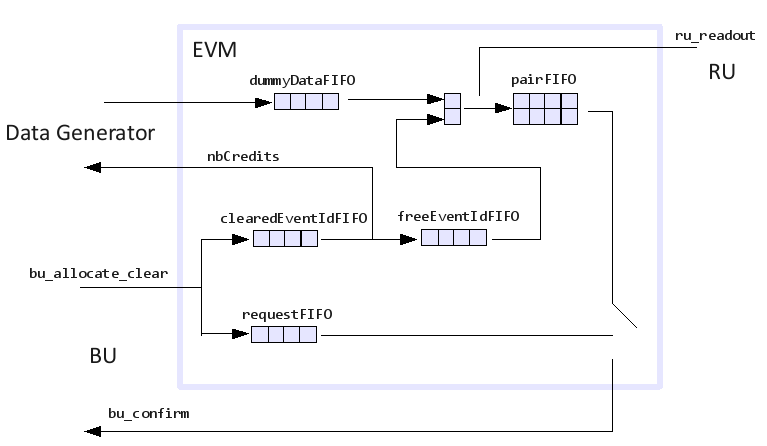
\includegraphics[width=0.90\textwidth]{figures/evm_behavior.png}
	\caption{Dynamic Behavior and Internal FIFOs of EVM}
	\label{fig:evm_behavior}
\end{figure}


\textbf{Step 1:} When the system is enabled the first event that the EVM receives is the $bu_allocate_clear$ event from the BU. Since there are no event requests available at the beginning, this event triggers the operation of the RU BUilder. Receipt of this event affects the $clearedEventId$ and $request$ FIFOs of EVM. The incoming event may be for a new event id request, be a request for release of a used event id, or be a request for both release of a used event id and a request for new event id. Upon reciept of the event, appropriate FIFOs are filled.

At the same time, the initial request for event data is sent to the DataGenerator component. Along with the request, a parameter called $nbCredits$ is sent. This denotes the number of available free event id slots in the builder. In this first step, the number of available free event id's is the size of the freeEventIdFIFO. 

\textbf{Step 2:} If there were a request to release an event id in the previous step, the freeEventIdFIFO is populated with the released event id.

\textbf{Step 3:} EVM asks for new event data with the number of released event id's as $nbCredits$ from the DataGenerator.

\textbf{Step 4:} DataGenerator sends the generated dummy event data to the EVM. Upon receipt of the data, dummyDataFIFO is filled with the event data. 

\textbf{Step 5:} If dummyDataFIFO and freeEventIdFIFO is not empty then pairFIFO is filled with the free event id from the freeEventIdFIFO and the event number from the dummyDataFIFO.

\textbf{Step 6:} When the conditions for Step 5 are satisfied EVM also sends $ru_readout$ event to RU with the event id/event number pair. 

\textbf{Step 7:} If the requestFIFO is filled with a request from BU, and the pairFIFO is filled with a Event Id/Event Number, then EVM sends $bu_confirm$ event.

Figure \ref{fig:evmmodel1} shows the DEVS model of EVM with states and input and output events.

\begin{figure}
	\centering
		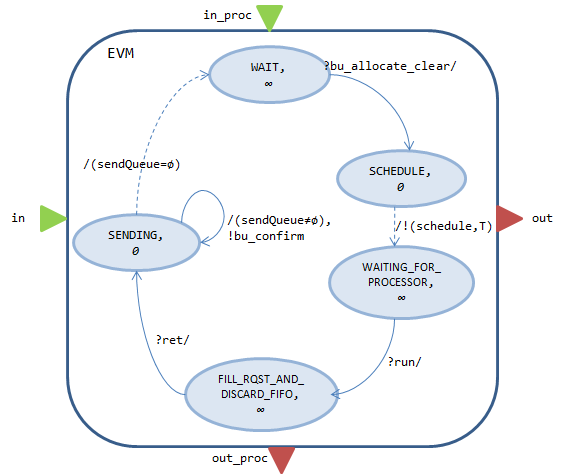
\includegraphics[width=0.95\textwidth]{figures/evmmodel1.png}
	\caption{EVM Model}
	\label{fig:evmmodel1}
\end{figure}

Initially, EVM is in WAIT state until an event is received. The events and state transition conditions are clearly indicated on the figure. EVM implements a queue called $sendQueue$ which is filled in when there is an output event to be sent out. 

\subsubsection{Readout Unit (RU)}
Readout unit is responsible for gathering the event data fragments and building super-fragments from them. Multiple fragments make up one complete event. DataGenerator generates dummy events with random fragment sizes. Figure \ref{fig:ru_behavior} shows the dynamic behavior of RU.

\begin{figure}
 \centering
 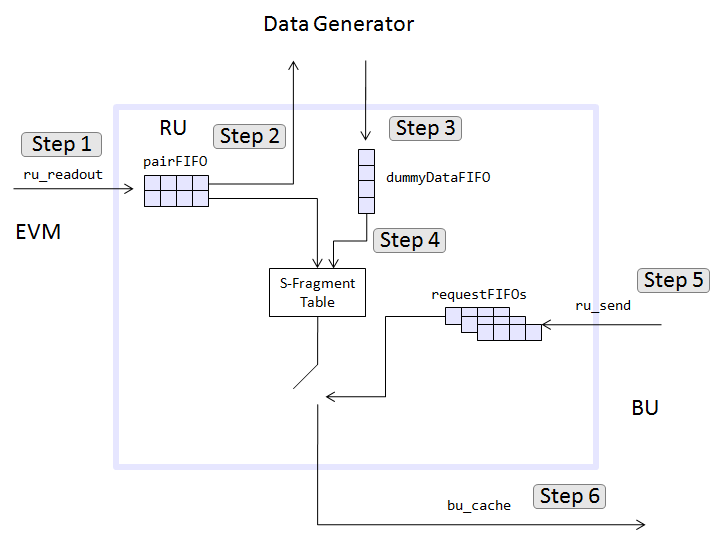
\includegraphics[width=0.90\textwidth]{figures/ru_behavior.png}
 % evm_behavior.png: 0x0 pixel, 0dpi, nanxnan cm, bb=
 \caption{Dynamic Behavior and Internal FIFOs of RU}
 \label{fig:ru_behavior}
\end{figure}


\textbf{Step 1:} The first step in the RU processing is the receipt of $ru_readout$ event from EVM. EVM sends RU a event id/event number pair for processing. RU populates its pairFIFO with event id/event number pair.

\textbf{Step 2:} RU asks the DataGenerator to send it the fragments of the event data that corresponds to the event number received from EVM.

\textbf{Step 3:} DataGenerator sends RU the number of blocks that  fragment for the specified event number is composed of. Upon reciept of the data the blockFIFO of RU is filled with the blocks received from the DataGenerator. In addition, at the same time, all blocks belonging to a single event are collected together to form event super-fragments.

\textbf{Step 4:} If the super-fragments are formed and pairFIFO is holding event id/event number pairs, then the table that is indexed by the event id from the pairFIFO and that holds all super-fragments is filled with super-fragment block.

\textbf{Step 5:} BU sends $ru_send$ event to request an event super-fragment to build. Upoxn reciept of the event, requestFIFO corresponding to the index of the BU that is requesting an event is populated.

\textbf{Step 6:} If any of the requestFIFOs is filled with a request, RU services the BU request with event super-fragments that are saved in the super-fragment table and sends out the $bu_cache$ event to BUs that requested an event.

Figure \ref{fig:rumodel1} shows the DEVS model of RU with states and input and output events.

\begin{figure}
	\centering
		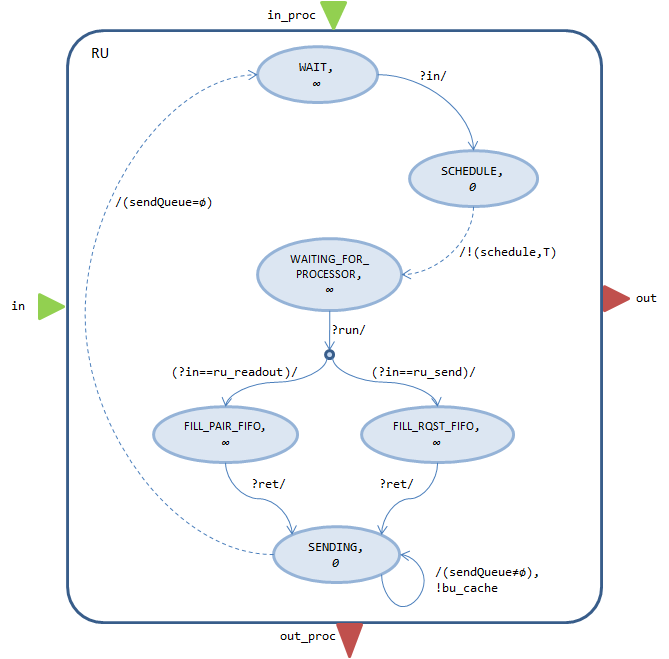
\includegraphics[width=0.95\textwidth]{figures/rumodel1.png}
	\caption{RU Model}
	\label{fig:rumodel1}
\end{figure}

\subsubsection{Builder Unit (BU)}
Builder Unit (BU) is responsible for building events  An event is composed of one super-fragment from coming from the DataGenerator and N RU super-fragments where N is the number of RUs. Figure \ref{fig:bu_behavior} shows the dynamic behavior of BU.

\begin{figure}
 \centering
 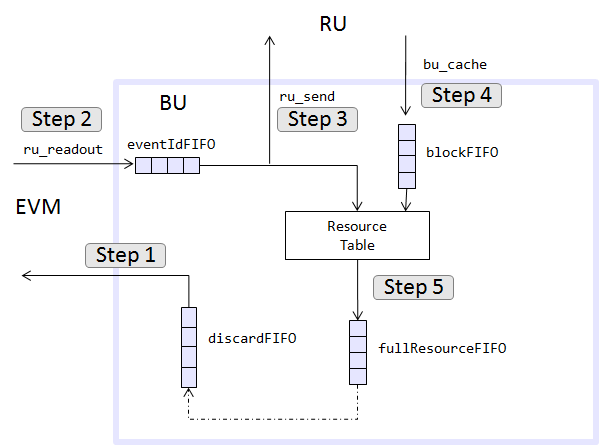
\includegraphics[width=0.90\textwidth]{figures/bu_behavior.png}
 % evm_behavior.png: 0x0 pixel, 0dpi, nanxnan cm, bb=
 \caption{Dynamic Behavior and Internal FIFOs of BU}
 \label{fig:bu_behavior}
\end{figure}


\textbf{Step 1:} As BU is enabled, the first action it takes is to send initial event requests to EVM. At this point the builder is completely available to build events. BU sends the event $bu_allocate_clear$ event to EVM.

\textbf{Step 2:} BU recieves the $bu_confirm$ event from EVM. Upon receipt of the event, BU fills in the eventIdFIFO with the id's of events that are assigned to the system by EVM. 

\textbf{Step 3:} If the eventIdFIFO is not empty, BU starts the construction of the event with the first event id in the eventIdFIFO and is ready to receive fragments of that event from RUs. At this point, BU sends out the $ru_send$ event to all RUs that are participating in the event building and asks for the fragments of the event that is under construction. Moreover, at this step, if a construction of an event is complete, then the fullResourceFIFO is filled by BU. This also increases the number of events built in the builder, and completes the lifecycle of an event id/event number pair.

\textbf{Step 4:} BU recieves the $bu_cache$ event from participating RUs. Upon receipt of this event, BU fills in the blockFIFO with blocks of event under construction.

\textbf{Step 5:} If there is an event data block in the blockFIFO then BU appends event block data to the previous blocks of the same event data. When  the event building is complete the number of events built in builder is incremented and the completed event block is put into the fullResourceFIFO. In addition, the completed event id ends its lifecycle and is pushed into the discardFIFO.

\textbf{Step 6:} In the simulation system, there is no Filter Unit to process the physical importance of those events. Instead the all the events are dropped after being completed and the number of events built in BU is incremented.

\textbf{Step 7:} If the discardFIFO is not empty then the used event id is recycled and $bu_allocate_clear$ is sent to EVM if the total number of events to be built has not been reached. 

Figure \ref{fig:bumodel1} shows the DEVS model of BU with states and input and output events. 


\begin{figure}
	\centering
		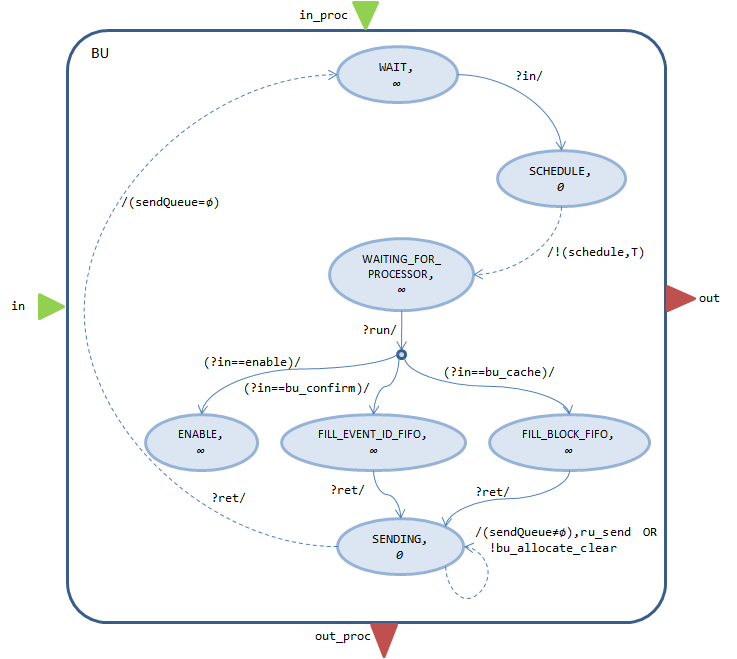
\includegraphics[width=0.95\textwidth]{figures/bumodel1.png}
	\caption{BU Model}
	\label{fig:bumodel1}
\end{figure}

\subsubsection{Peer Transport (PT)}
PeerTransport is the component that is responsible for transmitting messages between applications. Figure \ref{fig:pt_behavior} shows the dynamic behavior of the PeerTransport.

\begin{figure}
 \centering
 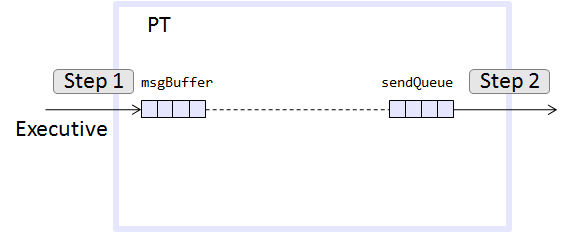
\includegraphics[width=0.90\textwidth]{figures/pt_behavior.png}
 % evm_behavior.png: 0x0 pixel, 0dpi, nanxnan cm, bb=
 \caption{Dynamic Behavior and Internal FIFOs of PT}
 \label{fig:pt_behavior}
\end{figure}

\textbf{Step 1:} PT receives $send$ event from the Executive. Upon receipt of the event, PT fills in the msgBufferFIFO. At this point, PT knows about the communication parties and the message that is being transmitted between them. 

\textbf{Step 2:} If the message buffer is not empty, PT puts the messages in the buffer into the sendQueueFIFO and sends out the message received from the Executive to all the applications. PT does not know the contents of the message or the event that is being transmitted. PT only transmits the message to all the applications and only the application with the id that matches the destination id of the message processes the event.

Figure \ref{fig:ptmodel1} shows the DEVS model of PT with states and input and output events.

\begin{figure}
	\centering
		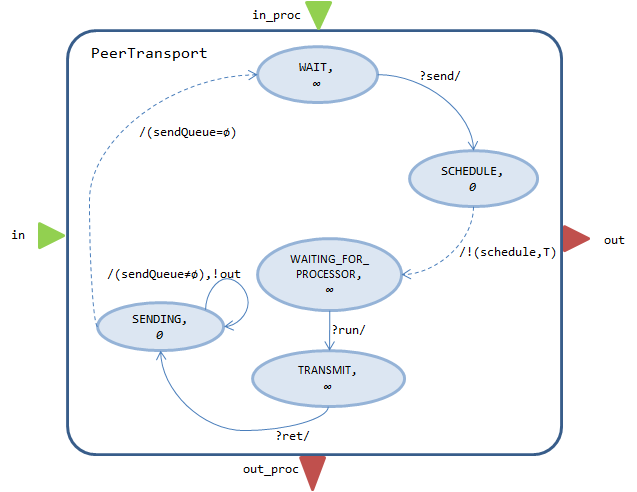
\includegraphics[width=0.95\textwidth]{figures/ptmodel1.png}
	\caption{PeerTransport Model}
	\label{fig:ptmodel1}
\end{figure}

\subsubsection{Executive}
Executive is the only application that resides in the middleware layer and is responsible with coordinating the communication of applications. Figure \ref{fig:executive_behavior} shows the dynamic behavior of the Executive.

\begin{figure}
 \centering
 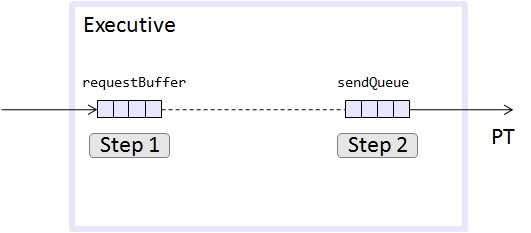
\includegraphics[width=0.90\textwidth]{figures/executive_behavior.png}
 % evm_behavior.png: 0x0 pixel, 0dpi, nanxnan cm, bb=
 \caption{Dynamic Behavior and Internal FIFOs of Executive}
 \label{fig:executive_behavior}
\end{figure}

\textbf{Step 1:} An application that needs to send an event to another application sends the event to the Executive. Upon receipt of the message from any application on its input port, the Executive saves the message into the requestBufferFIFO. 

\textbf{Step 2:} Executive knows about the available PeerTransports to use to send messages to the desired applications. Executive sends the $send$ event to the appropriate PT. 

Figure \ref{fig:executivemodel1} shows the DEVS model of Executive with states and input and output events. 

\begin{figure}
	\centering
		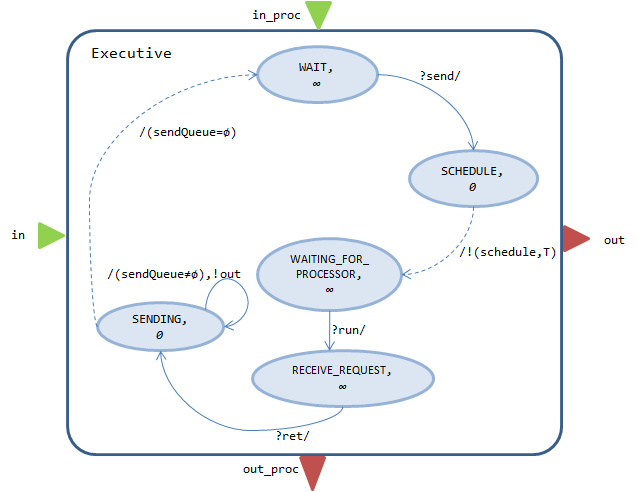
\includegraphics[width=0.95\textwidth]{figures/executivemodel1.png}
	\caption{Executive Model}
	\label{fig:executivemodel1}
\end{figure}

\subsection{Processor Model}
The experimental framework also includes a processor model to implement simple scheduling. Figure \ref{fig:Processor} shows the DEVS model of the processor along with it states, transition conditions and inputs and outputs.


\begin{figure}
	\centering
		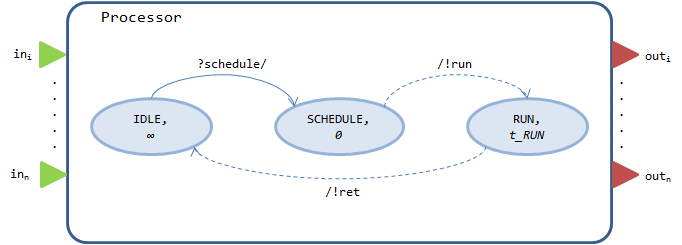
\includegraphics[width=0.99\textwidth]{figures/Processor.png}
	\caption{Processor DEVS Model}
	\label{fig:Processor}
\end{figure}

Processor receives a scheduling request from an application. Along with the scheduling request, application also sends the time it requests. The processor buffers all the scheduling requests. Then the ``$run$'' event is sent to the requesting application while the processor switches from the IDLE state to the RUN state. The life span of the RUN state of the processor becomes the amount of time requested by the application. Once the lifespan of the RUN state is elapsed, processor sends out the ``$ret$'' event to ask the application to return. Processor has several input and output ports. Every application has an input port connecting it to the processor, and there is one output port for every application to connect the processor output to the applications.

\subsection{Performance Aspect in Models}
DEVS models of applications are given in the previous sections. It's also important to note that some parameters related to the performance of the system are also captured in the application models. These parameters are mainly parameters of RU Builder applications. 

The XDAQ system is distributed as a software package by CERN which does not allow tuning of performance or modification of any performance related parameters. The tuning is done by the developers for only the case for which the system is going to be deployed for the experiment. However, for the purposes of this research, it was crucial to know the parameters which are highly probable to have an impact on the system performance. 

Upon conversations with XDAQ developers, it was made clear that so called packing parameters, and total number of blocks that make up a s-fragment are among the most important parameters that affect the performance of the system. In the original XDAQ system all packing parameters are set as $8$. Fragment sizes change during operation as different events have differing amounts of data. 

Packing parameters are captured in EVM and BU models. EVM has \textit{RU\_READOUT\_PACKING} parameter which determines how many requests need to be packed before sending a readout request to RUs. BU has \textit{EVM\_ALLOCATE\_CLEAR\_PACKING} which determines how many requests need to be packed before requesting or releasing an event id  and \textit{RU\_SEND\_PACKING} which determines how many requests need to be packed before sending s-fragment requests from RUs.

In addition to the packing parameters, BU model captures $blockFIFOCapacity$, $requestFIFOCapacity$, and $maxEvtsUnderConstruction$ which determines the maximum number of events that can be constructed in BU.

Varying event data block sizes are not captured in the application models but rather in the data generator which is explained in the next section. 

\section{Input Data Generator}
The experiment platform and the simulation engine is driven by a dummy input data generator. As stated in the previous section, differing event data fragment sizes are generated by the dummy data generator and fed into the system. 

The input data generator is modeled both in TSDML and simulation. The important aspects of the input data generator that are captured in TSDML are:

\begin{itemize}
	\item RandomDistribution: Enables selection of the type of distribution that is wanted to be used
	\item BlockSize: According to \cite{CMSTDR}, block size of an event is 4 kB and has to be captured in the so that it can be varied if needed. Number of blocks in s-fragment is a statical distribution since different events have different amounts of data \cite{CMSTDR}.
	\item NumberOfDataSources: In the CMS system, there are actually 8 total number of data sources. In order to simulate this behavior, this is also captured in TSDML.
	\item EventSizeMean: Average size of an event is 1 MB \cite{CMSTDR}. This is captured in the TSDML so that event mean can be varied and the system can be tested with varying mean event sizes.
	\item EventSizeSigma: Standard deviation for the event size.
\end{itemize}

Capturing the input data generator abstractions in TSDML also enables varying the input data parameters using a sweeper. This is illustrated in Figure \ref{fig:SweepInputGenerator}.

\begin{figure}
	\centering
		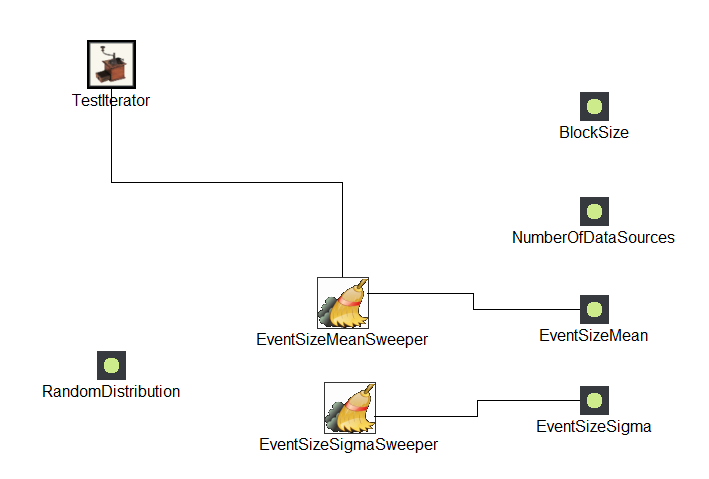
\includegraphics[width=0.70\textwidth]{figures/SweepInputGenerator.png}
	\caption{Sweeping EventSizeMean and EventSizeSigma}
	\label{fig:SweepInputGenerator}
\end{figure}

The core part of the input data generator is implemented as part of the simulation. However, it is not implemented as a DEVS model and rather implemented as a stand alone component. The type of random distribution is selected from the TSDML model and can be normal, log normal, exponential or uniform. Boost Random library is used to generate a random distribution \cite{boost}. For the random distribution generation Mersenne Twister random number generator is used. The following code snipped demonstrates how a log normal distribution was generated:

\begin{verbatim}
	//Create a Mersenne twister random number generator
	static mt19937 rng( static_cast<unsigned> (time(0)) );
	//Select distribution
	lognormal_distribution<double> lognorm_dist(_eventSizeMean, _eventSizeSigma);
\end{verbatim}

In addition to generating random distribution, input data generator component is also responsible for generating event numbers and super fragments to be consumed by the system. Figure \ref{fig:DataGenerator} shows how the input data generator component fits with the rest of the DEVS models.

\begin{figure}
	\centering
		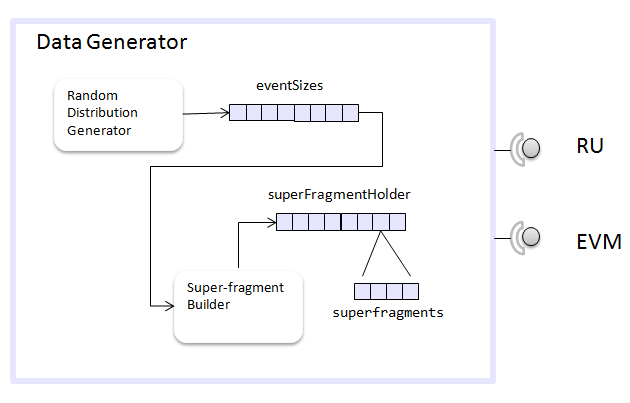
\includegraphics[width=0.65\textwidth]{figures/DataGenerator.png}
	\caption{Input Data Generator Component View}
	\label{fig:DataGenerator}
\end{figure}

Input data generation is triggered by EVM. Number of random event sizes based on the selected distribution is generated. The total number of event sizes generated depends on the total number of events that can be built by XDAQ. EVM also triggers the super-fragment building from the generated event sizes. A super-fragment is a collection of fragments. In XDAQ system, an event is composed of several blocks (4KB each) because of the distributed nature of the system. The goal of super-fragment building is to collect all blocks of an event into one chunk called a super-fragment. The input data generator represents a super-fragment as a structure with the following fields:

\begin{itemize}
	\item Event Number
	\item Super-fragment Size = Event Size / Number of Super-fragments
	\item Number of Blocks in Super-Fragment = Super-Fragment Size / Block Size
	\item Super-fragment Number
	\item Event data blocks
\end{itemize}

In the above structure, the fields Super-fragment size and Number of Blocks In Super-fragment depend on the random event size data generated by the input generator. Event Size is the size that is generated with selected random distribution. Number of Super-fragments equals to the total number of RUs in the system. As can be observed, super-fragment is distributed equally among all RUs. 

In summary, the input data generator generates input event data that is distributed according to a selected random distribution type and provides a representation of event data in the form of a super-fragment. A super-fragment for a specific event number/event id pair is what is consumed by the simulation engine during a test run.

\section{Communication Interfaces Between Applications}

\subsection{EVM-BU Interface}

EVM and BU has two way interface. Figure \ref{fig:evm-bu} shows the events passed between EVM and BU.
\begin{figure}
	\centering
		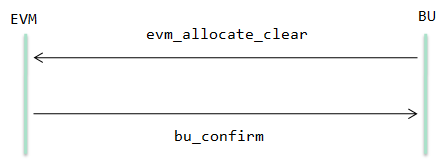
\includegraphics[width=0.85\textwidth]{figures/evm-bu.png}
	\caption{EVM-BU Interface Diagram}
	\label{fig:evm-bu}
\end{figure}

BU starts the interaction between itself and EVM by sending event requests by sending the \textit{evm\_allocate\_clear}. The message format of the communication between EVM and BU is as follows: 
\begin{quote}
	address\#sourceId\#destinationId\#event\#data
\end{quote}

BU sends the following data along with the event:

\begin{itemize}
	\item \textbf{buAddress}: The IP address of the computer that the BU is running on
	\item \textbf{buId}: Unique identifier of the source application, BU
	\item \textbf{destinationId}: Unique identifier of the destination application
	\item \textbf{eventName}: Name of the event which is \textit{evm\_allocate\_clear} in this case
	\item \textbf{data}: Actual request message which consists of the request.
\end{itemize}

In order to form the request data, BU sets the following parameters:
\begin{itemize}
	\item BU Id: The unique identifier of the BU that is making the request.
	\item Number of Requests Packed: BU does not send one request at a time but packs multiple requests into one request. The total number of requests are sent as part of the request data.
	\item Request type: $0$ means event id request, $1$ means releasing an event id and requesting another, and $2$ means releasing an event id.
	\item Event Id: Event id to be released. If requesting an id, this is not need to be set.
	\item Event Number: Event number that is associated with the released event id. If requesting an id, this is not need to be set.
	\item Resource Id: The resource id of the BU that is making the request.
\end{itemize}

EVM receives the request from the BU and acts on it. As a result, EVM sends out the \textit{bu\_confirm} event to the requesting BU. EVM sends the following data along with the event:

\begin{itemize}
	\item \textbf{evmAddress}: The IP address of the computer that the EVM is running on
	\item \textbf{evmId}: Unique identifier of the source application, EVM
	\item \textbf{buId}: Unique identifier of the destination application, BU
	\item \textbf{event}: Name of the event which is \textit{bu\_confirm} in this case
	\item \textbf{data}: The confirmation message to BU
\end{itemize}

In order to for the confirmation data, EVM sets the following parameters:

\begin{itemize}
	\item \textbf{Event Number (eventNumber)}: Event number assigned to BU
	\item \textbf{Number of Blocks In super-fragment (nbBlocksInSuperFragment)}: Number of blocks that make up the sfragment
	\item \textbf{Block Number (blockNb)}: The position of the current block in the sfragment. It is set as $0$ at this time.
	\item \textbf{Event Id (eventId)}: Event id that is assigned to the BU.
	\item \textbf{Super-fragment Number (superFragmentNb)}: The number of the super-fragment in the block. Set as $0$ for the first set of data.
\end{itemize}


\subsection{EVM-RU Interface}

EVM and RU has a one way interface. Figure \ref{fig:evm-ru} shows the interaction between EVM and RU.

\begin{figure}
	\centering
		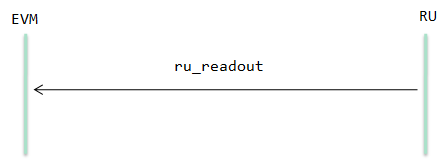
\includegraphics[width=0.85\textwidth]{figures/evm-ru.png}
	\caption{EVM-RU Interface Diagram}
	\label{fig:evm-ru}
\end{figure}

EVM sends RUs the \textit{readout} event. The message format of the communication between EVM and RU is as follows:

\begin{quote}
	address\#sourceId\#destinationId\#event\#data
\end{quote}

EVM sends the following data along with the event:

\begin{itemize}
	\item \textbf{Number of Elements Packed}: Total number of read out requests that is packed. EVM doesn't send events one by one. Multiple read out requests are sent.
	\item \textbf{Event Id}: Event id to be read out from the data generator.
	\item \textbf{Event Number}: Event number of the data that is read out from the data generator.
\end{itemize}


\subsection{BU-RU Interface}

BU and RU has a two way interface. Figure \ref{fig:bu-ru} shows the interaction between BU and RU.

\begin{figure}
	\centering
		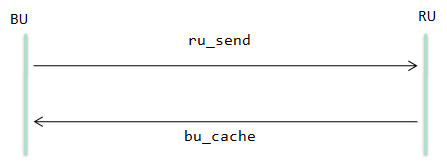
\includegraphics[width=0.85\textwidth]{figures/bu-ru.png}
	\caption{BU-RU Interface Diagram}
	\label{fig:bu-ru}
\end{figure}

The message format of the communication is as follows:

\begin{quote}
	address\#sourceId\#destinationId\#event\#data
\end{quote}

BU sends RU the \textit{ru\_send} event. BU sends the following data along with the event:

\begin{itemize}
	\item \textbf{Event Id}: Event id of the event that BU is requesting
	\item \textbf{Event Number}: Event number of the event that BU is requesting
	\item \textbf{BU Resource Id}: Resource id of the BU that is going to build the event
	\item \textbf{BU Id}: Unique identifier of BU that is requesting the event data
\end{itemize}

RU sends BU the ''\textit{bu\_cache}'' event. RU sends the following data along with the event:

\begin{itemize}
	\item \textbf{Block Number}: The current block number of the event data in the data chain
	\item	\textbf{BU Resource Id}: Resource id of the BU that is going to build the event
	\item \textbf{Event Id}: Event id of the event that BU is requesting
	\item \textbf{Event Number}: Event number of the evet that BU is requesting
	\item \textbf{Number of Blocks in Super-fragment}: Total number of blocks that make up the s-fragment
	\item \textbf{Super-fragment Number}: The current s-fragment number in the s-fragment chain
\end{itemize}


\subsection{Application-Executive-PT Interface}

The Executive has one way interface with all the applications. Figure \ref{fig:exec-pt} shows the interaction between applications, executive, and peer transport.

\begin{figure}
	\centering
		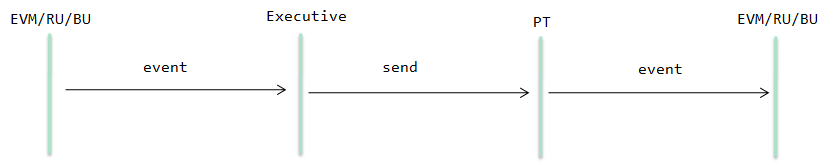
\includegraphics[width=1.0\textwidth]{figures/exec-pt.png}
	\caption{Executive-Peer Transport Interface Diagram}
	\label{fig:exec-pt}
\end{figure}

Since applications need to go through the Executive to pass data to other applications, the above mentioned communication should go through the Executive. 

Executive sends PT the \textit{send} event. The message format is the same as given above since Executive does not need any extra information and transmit the data without making any modifications to it. Executive sends the data received from the application along with the event. 

PT has one way interface with the the applications. PT sends the destination application the original event that is being transmitted between the applications. PT does not also make any modifications to the data being transmitted.

\subsection{Application-Processor Interface}

Processor has two-way interface with all the applications. All applications go through the Processor for scheduling processing time. Figure \ref{fig:processor-app} shows the interaction between applications and the Processor.

\begin{figure}
	\centering
		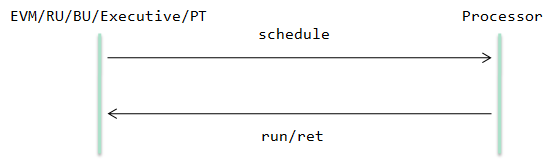
\includegraphics[width=0.85\textwidth]{figures/processor-app.png}
	\caption{Processor-Application Interface}
	\label{fig:processor-app}
\end{figure}

Applications send the Processor the \textit{schedule} event when they request scheduling. Applications send the requested amount of time along with the event.

Processor sends the requesting application the \textit{run} event to notify it to start running. Processor does not pass any data along with the event.

Processor sends the scheduled application the \textit{ret} event to notify that the time is up and the application should return. Processor does not pass any data along with the event. 

\section{Test Generation from TSDML Models}
In Chapter \ref{Chapter:Methodology}, a description of Test Series Definition Modeling Language (TSDML) and how different components of the system under test can be modeled. This section will give an example implementation of TSDML for test generation and provide more details on the process which was shown in Figure \ref{fig:SimulationRun} in Chapter \ref{Chapter:Methodology}.

\subsection{Constructing a Test Series Definition}
In order to demonstrate an example TSDML model, construction of a test series definition for generating several test cases to experiment with different event sizes will be described from the ground up. 

\subsubsection{Application Types}
In order to construct a test series definition, applications that will be used in the definition should be created in the Type Library. Applications that are required for the test system are EVM, BU, RU and PT. The entities that are required to model an application type is already described in Section \ref{Section:TSDML} of Chapter \ref{Chapter:Methodology}.

Parameters of application types that are used in application type models come from \cite{rubuilder}. Some changes to the organizations of these parameters where appropriate to help with test generation. All application types have bi-directional communication ports to all other applications. In addition, application types include positive and negative probes as well. Figure \ref{fig:EVMModel} shows the modeling of EVM application as an application type.

\begin{figure}
	\centering
		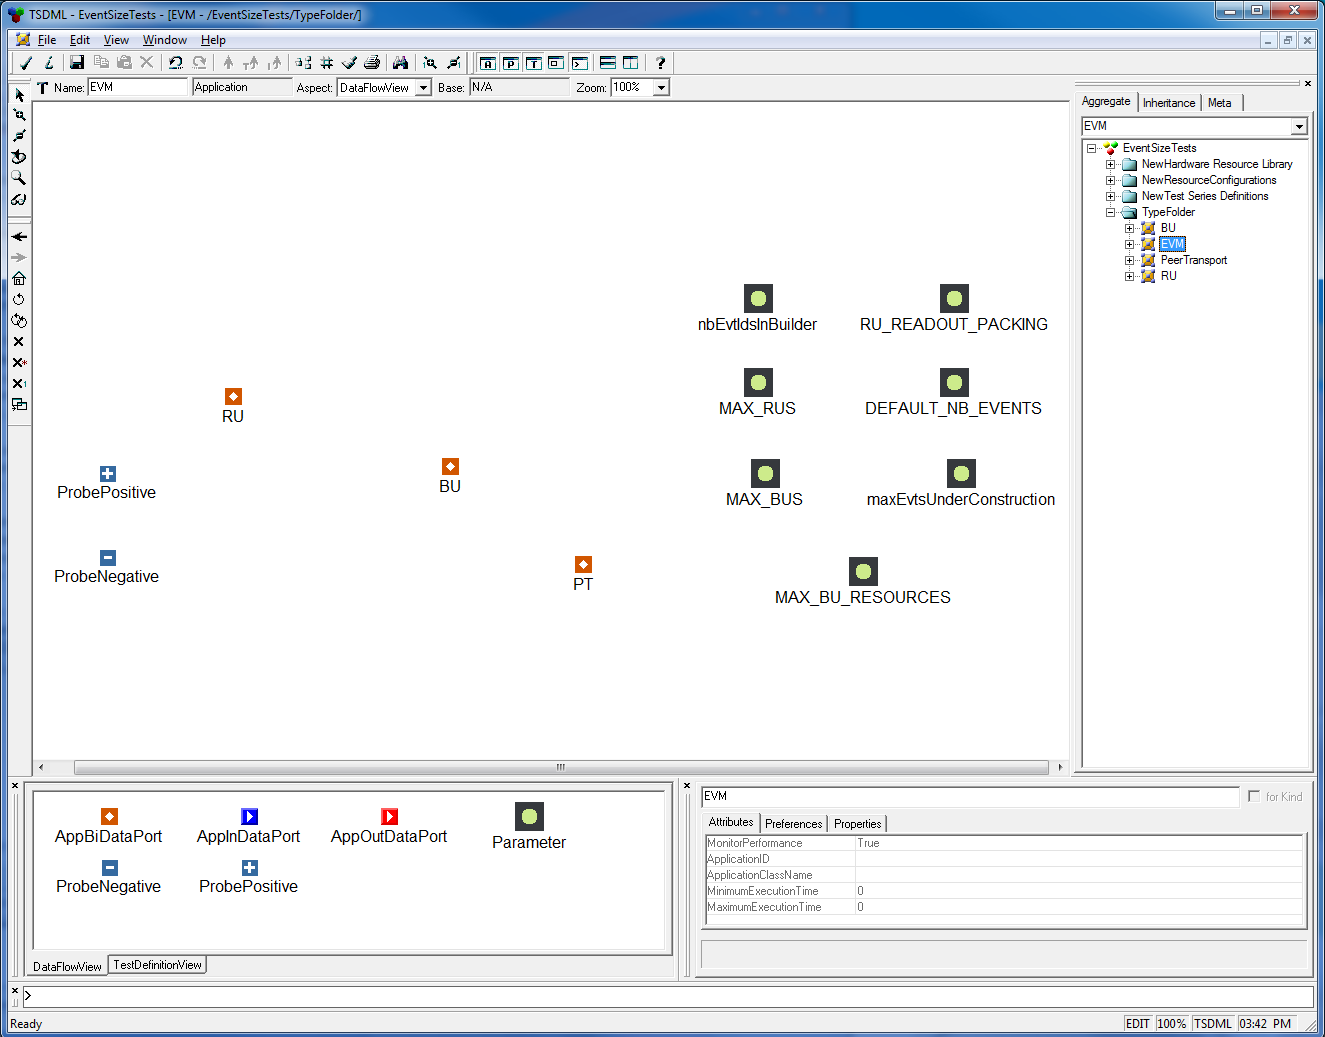
\includegraphics[width=0.95\textwidth]{figures/EVM_tsdml.png}
	\caption{Application Type Model for EVM}
	\label{fig:EVM_tsdml}
\end{figure}

It's important to note that application types are modeled without any parameter values. This way, when an application type is used (instantiated) in a test series definition it can be specialized by changing its parameter values. All other application models are similar to EVM.

\subsubsection{Test Series Definition}
The test series definition is the main part of the design as the name implies. There are three different aspects that need to be modeled to complete a test series definition so that test cases can be generated.

In a test series definition, several ways exist to generate test cases to experiment with the system in different ways. One way to generate different series of test cases is to change the structure of the system using replicators. This is done in the \textit{\textbf{Test Series Definition View}}. The Test Series Definition view is where the applications that were defined in the application library are used. Applications from the type library are sub-typed so that values for application parameters can be manipulated as desired. In addition, this way, it is not possible to make changes to the application type, e.g. no parameter or port can be deleted. This is to make sure that the same application type is used in all test series definitions with only the desired parameter value changes. 

\begin{figure}
	\centering
		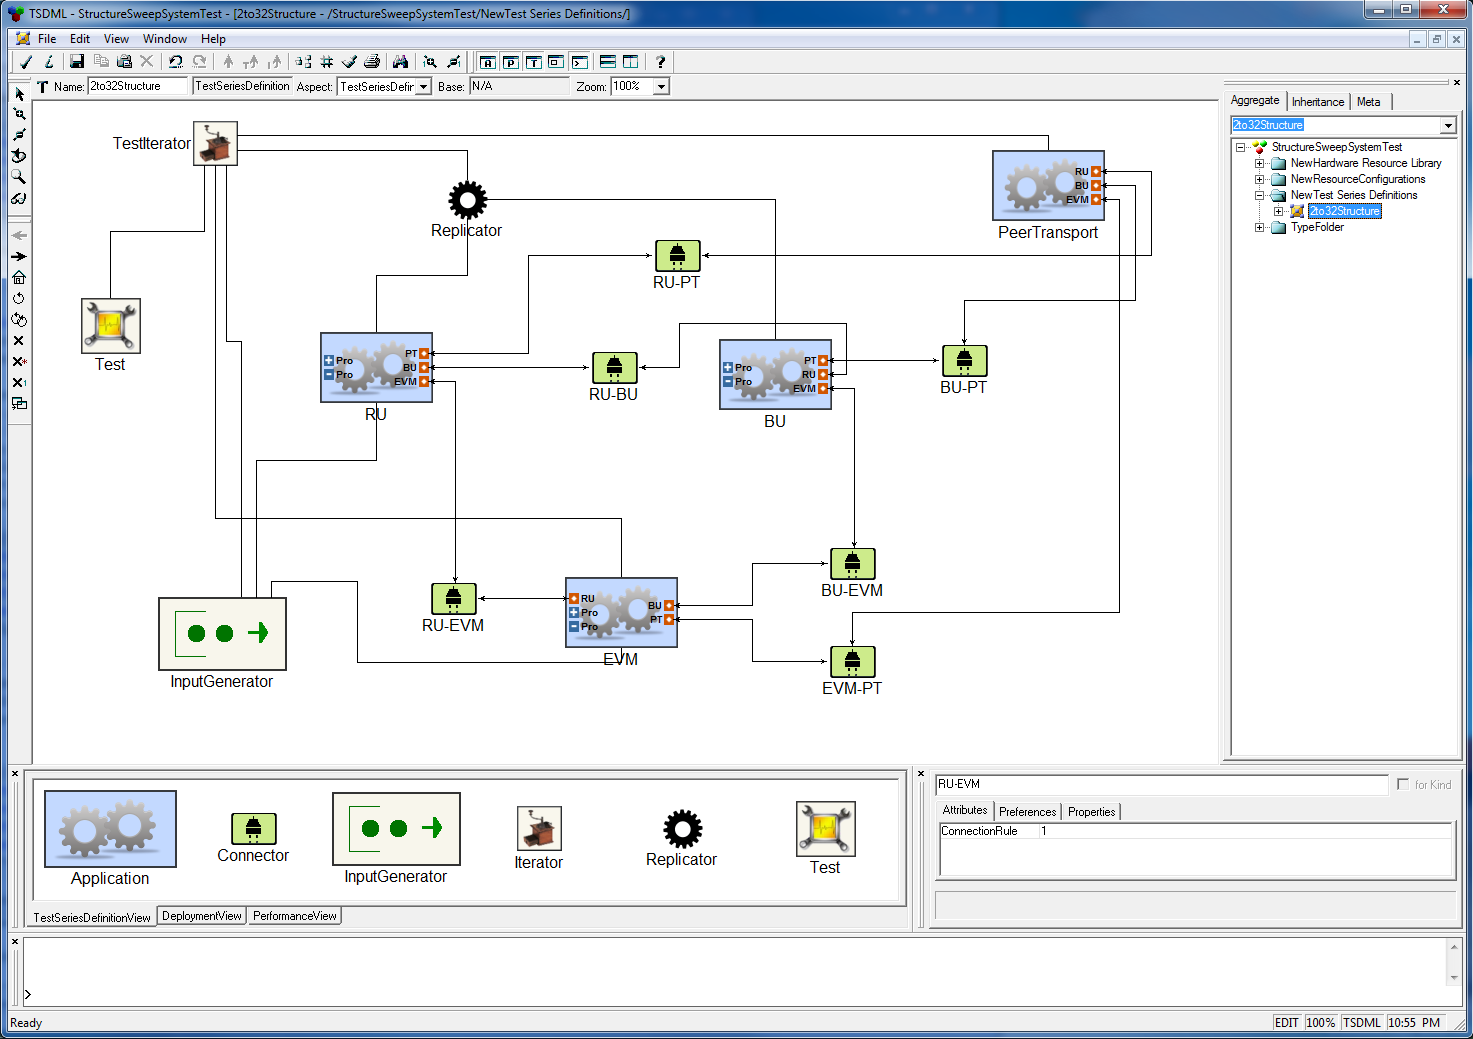
\includegraphics[width=0.90\textwidth]{figures/TSDModel.png}
	\caption{Test Series Definition View of a Test Series Definition with Replicators}
	\label{fig:TSDModel}
\end{figure}

Figure \ref{fig:TSDModel} shows how the Test Series Definition View looks.Sub-types of the applications already modeled in the type library are used in the test series definition. It can be seen from Figure \ref{fig:TSDModel} that there is an iterator connected to a replicator which is connected to applications RU and BU. This denotes that there will be as many test cases generated from this test series definition as the value of the Iterator. Moreover, in each of these test cases, applications RU and BU will be replicated by the value of the replicator. In this specific example, in each test case the instances of RU and BU will be doubled. Figure \ref{fig:TSDItRep} shows the values of the Iterator and the Replicator. It's important to note that only the applications RU and BU will be replicated in generated test cases since the Replicator is only attached to these applications. 

\begin{figure}
	\centering
		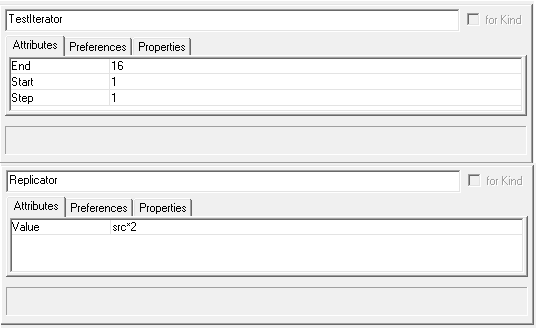
\includegraphics[width=1.00\textwidth]{figures/TSDItRep.png}
	\caption{Iterator and Replicator Values}
	\label{fig:TSDItRep}
\end{figure}

In the replication process, in addition to application instances, connections between applications need to be replicated as well. For this purpose, several Connectors are used to connect the applications on their bi-directional ports. In this test series definition, all applications are connected to each other. As can be seen in Figure \ref{fig:ConnTSD}, the Connector between applications RU and BU is called RU-BU and its connection rule is set to "`1"'. This means that all instances of RU and BU in generated test cases are connected to each other. The connection rules of connectors RU-PT, RU-EVM, BU-PT, BU-EVM, and EVM-PT are also set to "`1"'. However, since the Replicator is not connected to applications PT, EVM, and BU there will always be only one instance of these applications, which are connected to each other, in all generated test cases. Another example of setting different connection rules was explained in Section \ref{Section:TSDML} of Chapter \ref{Chapter:Methodology}. 

\begin{figure}
	\centering
		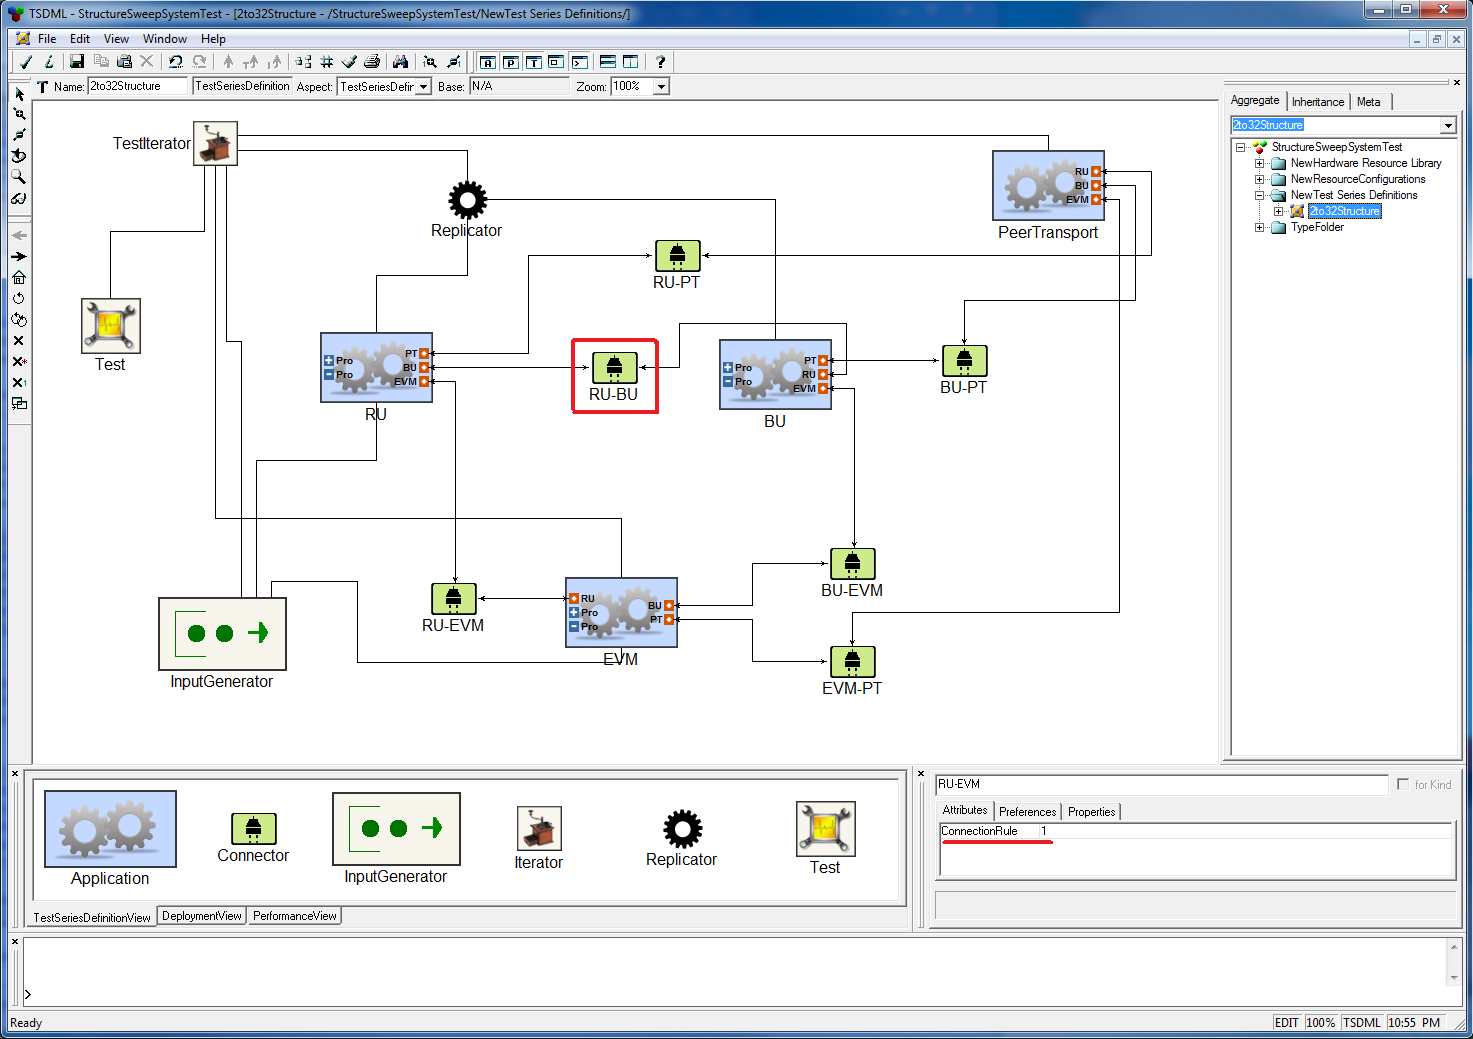
\includegraphics[width=0.95\textwidth]{figures/ConnTSD.png}
	\caption{Connection Rule is 1: All instances are connected}
	\label{fig:ConnTSD}
\end{figure}

\begin{figure}
	\centering
		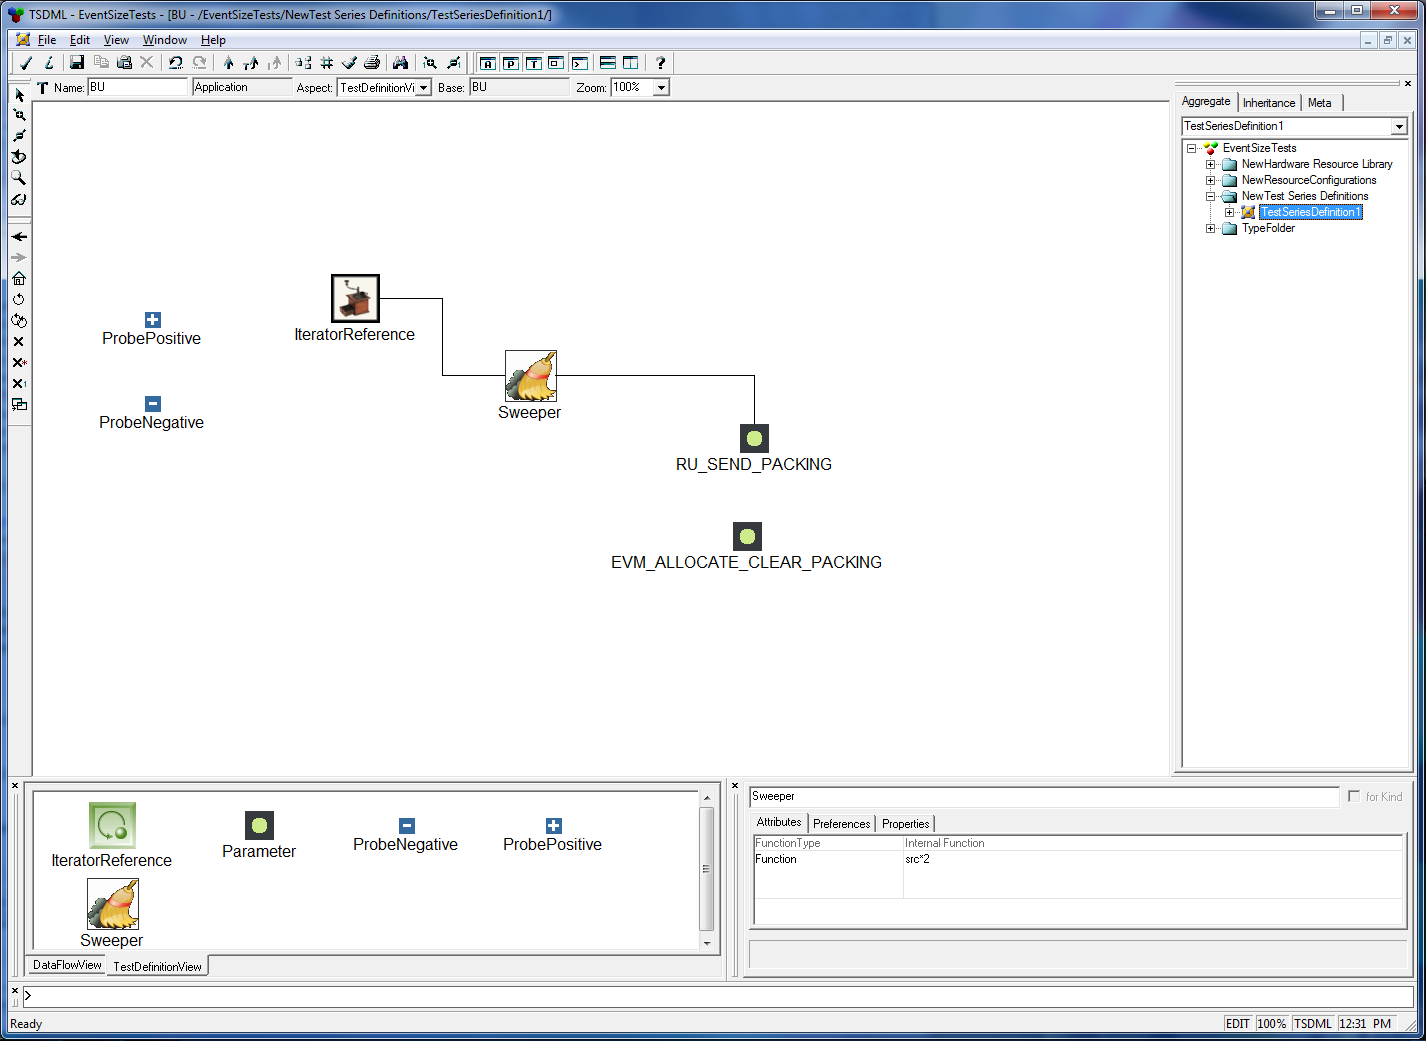
\includegraphics[width=1.00\textwidth]{figures/TSDSweep.png}
	\caption{Sweeping Application Parameter Value}
	\label{fig:TSDSweep}
\end{figure}

Another way to generate different series of test cases is to vary ("`\textit{sweep}"') application parameter values for each generated test case. This can be done using a Sweeper. Sweeper is present in the Test Definition View of an application model in the Test Series Definition. Figure \ref{fig:TSDSweep} shows usage of Sweeper to generate test cases with varying value for the $RU\_SEND\_PACKING$. The Sweeper has a function to double the value of $RU\_SEND\_PACKING$. Sweeper is also connected to a reference to the Iterator of the Test Series Definition which ensures that the value of the parameter will be doubled for each generated test case. 

Similar to varying application parameter values, Sweeper can also be used to vary parameters of the Input Generator of the Test Series Definition. This is especially useful to experiment with varying event sizes. Figure \ref{fig:TSDInput} demonstrates how this is done.  As can be seen in the figure, for each generated test case, mean of event size will be increased by 4 megabits.

Also in the same figure, the RandomDistribution entity can be seen. Input Generator will create random event sizes with the selected random distribution type.

\begin{figure}
	\centering
		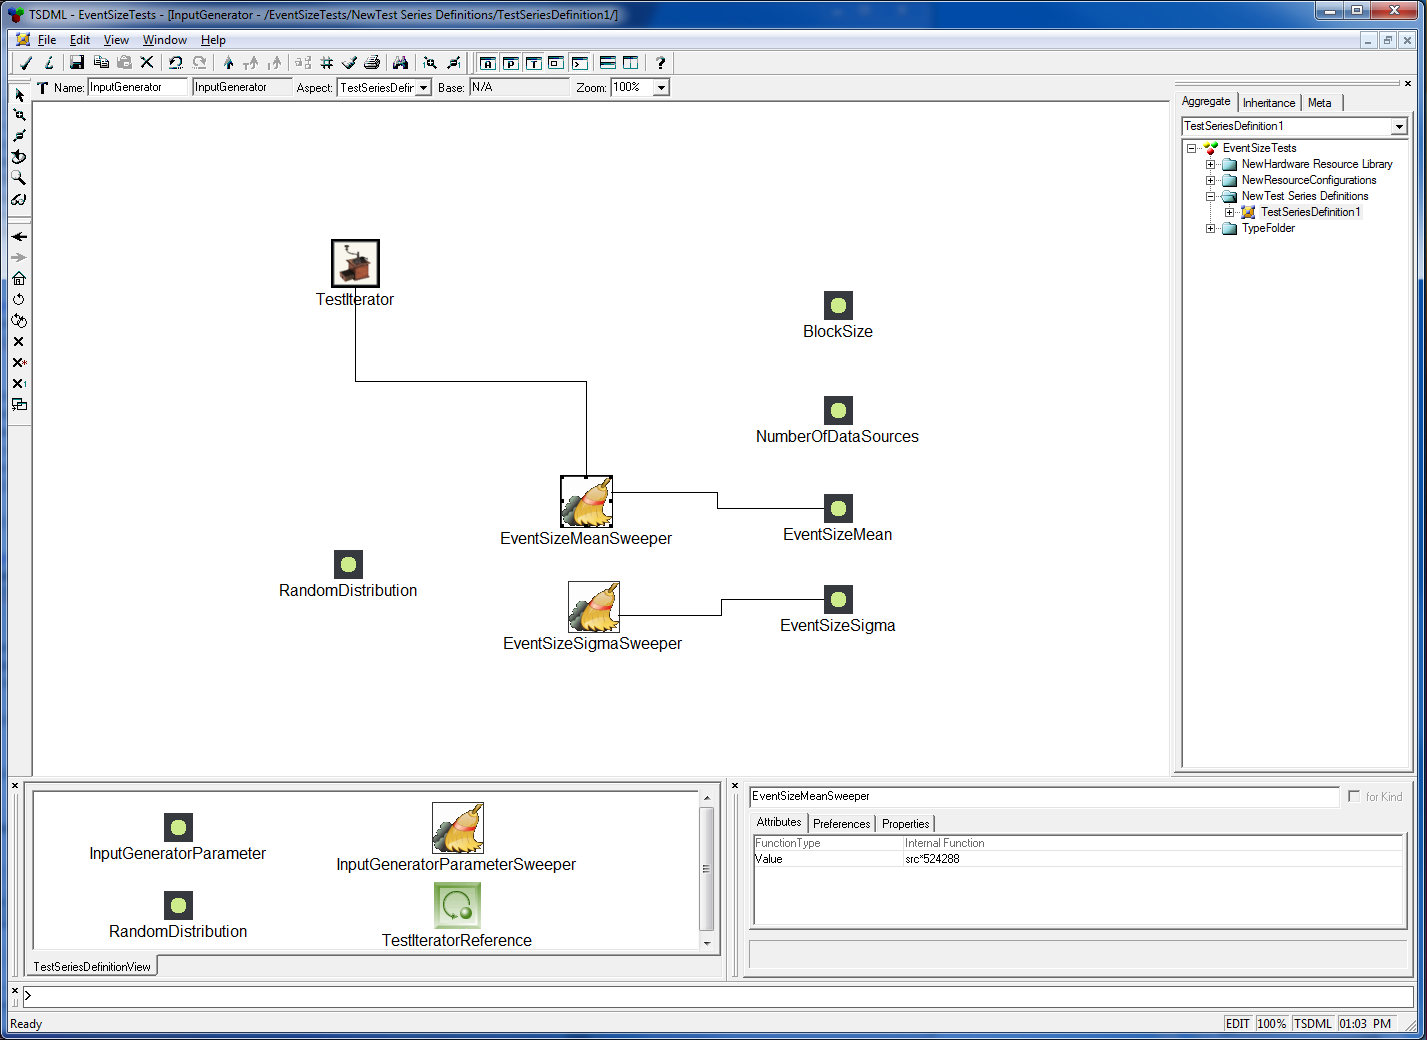
\includegraphics[width=1.00\textwidth]{figures/TSDInput.png}
	\caption{Sweeping Event Size in Input Generator}
	\label{fig:TSDInput}
\end{figure}

So far a test series definition is defined from the Test Series Definition View which enabled creating variations on the system structure and behavior to generate series of test cases. Another aspect of creating a test series definition is deployment. The \textit{\textbf{Deployment View}} enables deploying the system. In order to start a deploying the applications, a Node in Resource Library needs to be modeled. Figure \ref{fig:TSDNode} shows a simple model of a node in the resource library.

\begin{figure}
	\centering
		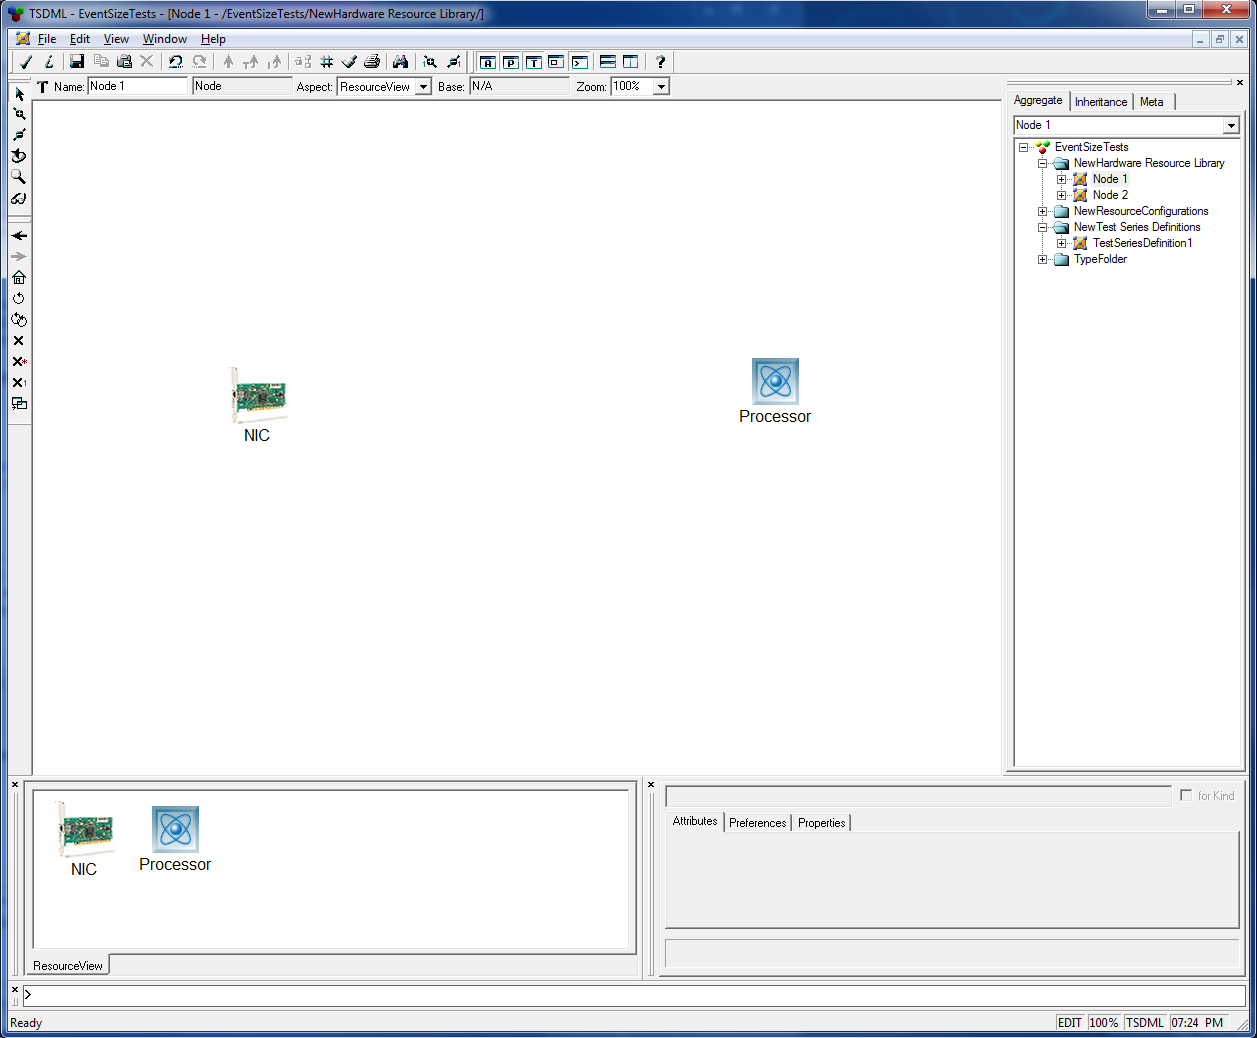
\includegraphics[width=1.00\textwidth]{figures/TSDNode.png}
	\caption{Model of a Node in Resource Library}
	\label{fig:TSDNode}
\end{figure}

Figure \ref{fig:TSDDeploy} shows a possible deployment for the test series definition under construction. The deployment view has a reference to the node that is created in the resource library. All the applications that were modeled in the Test Series Definition view are also visible in Deployment View and they are all connected to the Executive. The Executive represents the middleware layer which applications need to be deployed on in order to operate. The Executive also needs to be deployed on a node through a port on which it will run. As can be seen in Figure \ref{fig:TSDDeploy}, the Executive is connected to the Port which is connected to the NIC of Node1. It's important to point out that Port is a logical entity and models the endpoint which will be available to run the Executive on Node1.

\begin{figure}
	\centering
		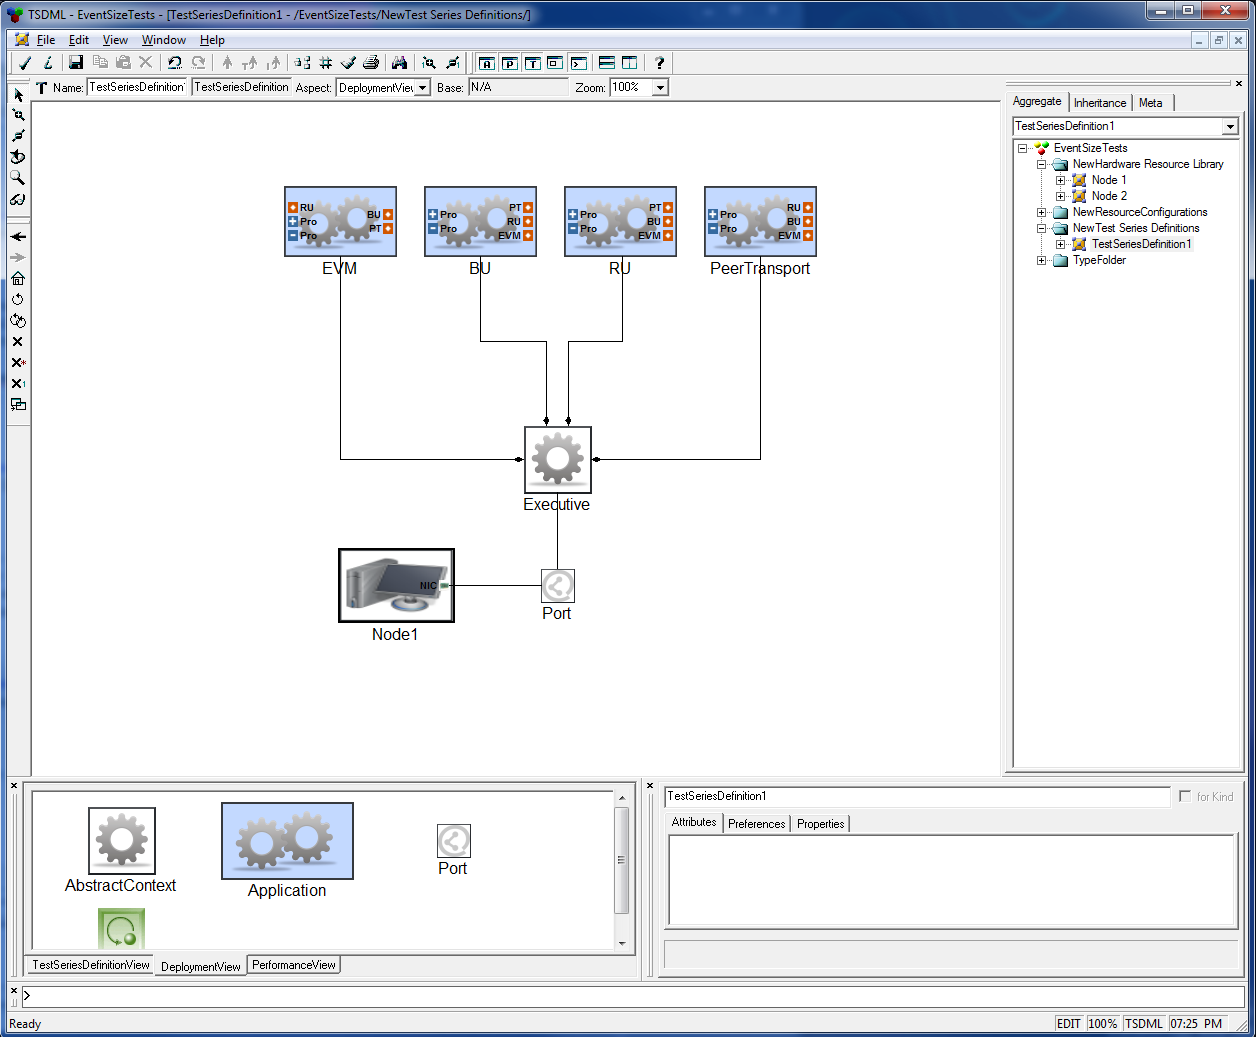
\includegraphics[width=1.00\textwidth]{figures/TSDDeploy.png}
	\caption{Deployment View of Test Series Definition}
	\label{fig:TSDDeploy}
\end{figure}

Test Series Definition View and Deployment View covered the behavioral/configuration and deployment aspects of the test series definition. \textit{\textbf{Performance View}} is where the performance related aspects are added. The main entity in the Performance View is the Performance Probe. Figure \ref{fig:TSDProbe} shows how performance probes are connected to indicate measurement points.

\begin{figure}
	\centering
		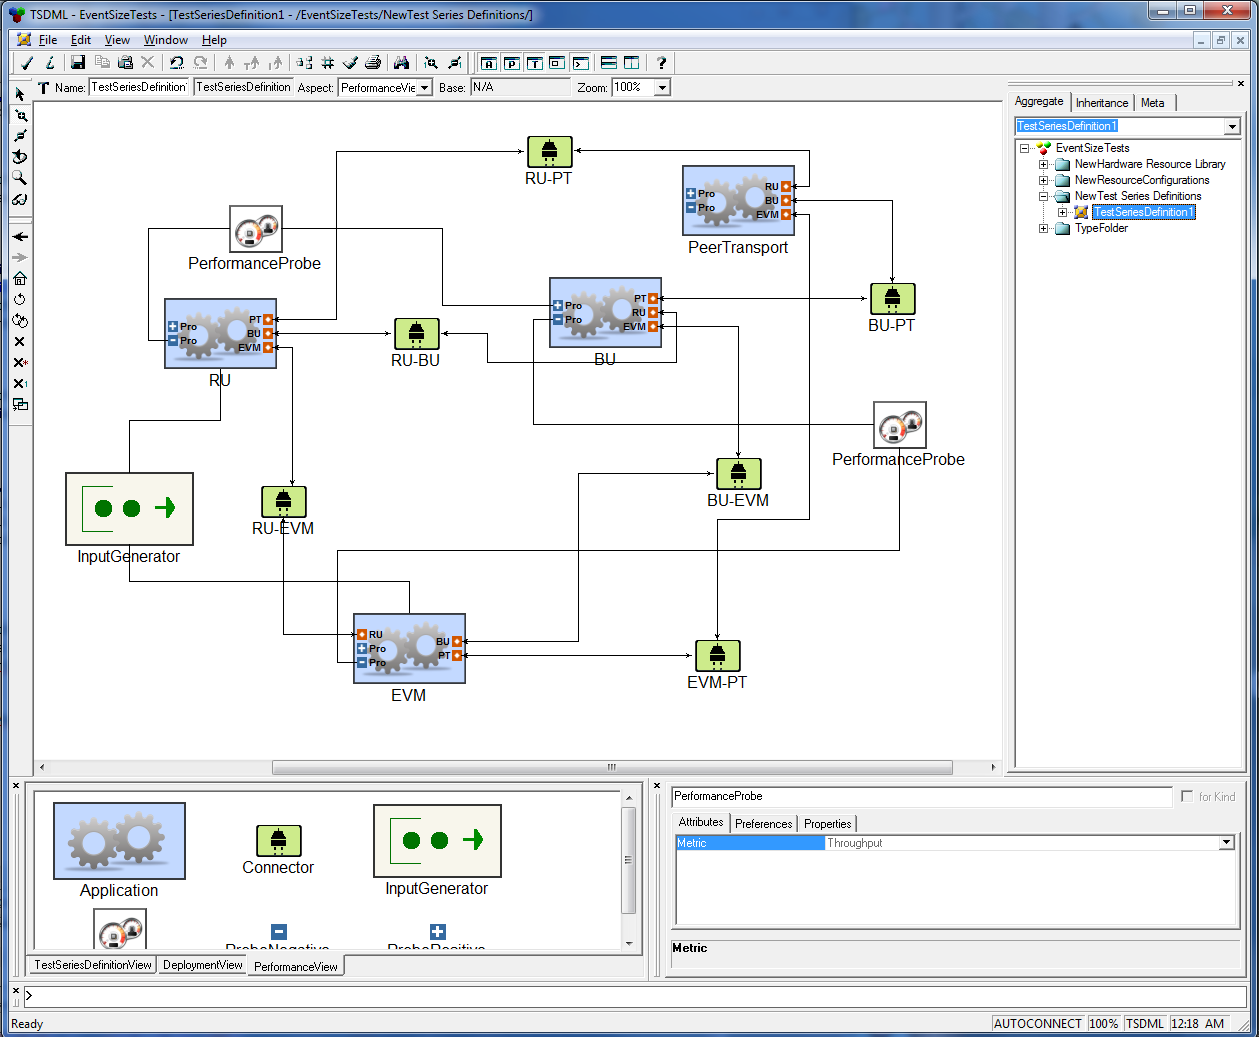
\includegraphics[width=1.00\textwidth]{figures/TSDProbe.png}
	\caption{Performance View of Test Series Definition}
	\label{fig:TSDProbe}
\end{figure}

In this specific example, one performance probe is connected to a negative probe end of application RU and the positive probe end on the application BU. This denotes that a performance measurement for a selected metric will be made between the output of RU and the input of BU. Another performance probe is connected between the negative probe end of application BU and positive probe end of application EVM. This denotes that a performance measurement for a selected metric will be made between the output of the application BU and the output of EVM. Figure \ref{fig:TSDProbeAdv} shows a more through use of performance probes.

\begin{figure}
	\centering
		\includegraphics[width=1.00\textwidth]{figures/TSDProbeAdv.png}
	\caption{Metric Choices for Performance Probe}
	\label{fig:TSDProbeAdv}
\end{figure}

\subsection{Test Case Generation}
Application simulation models and TSDML models are created. These models represent the behavioral, structural, and performance aspects of the system under test under the described abstractions. As described throughout this document, TSDML models will be used for generating series of test cases to be executed on the DEVS simulation engine. 

Test cases that will be generated from test series definitions in TSDML are XML configuration files that will configure the simulation engine with the information captured in the test series definitions. Figure \ref{fig:TSDTestGen1} shows the process of test case generation. The XML configurations generated from test test series definition need to be fed into the simulation engine.

\begin{figure}
	\centering
		\includegraphics{figures/TSDTestGen1.png}
	\caption{Test Generation Process}
	\label{fig:TSDTestGen1}
\end{figure}

The interaction between test cases and the simulation engine requires a test case format that can be read by the simulation engine. For this purpose, a schema for XML test cases were created. Figure \ref{fig:TSDConfigSchema} shows the test schema of the test cases that will be generated by the test series definition TSDML and read by the simulation engine. As can be seen in the figure there are five main tags which collect the information in the model:

\begin{enumerate}
	\item \verb|<test>|: the root of the test case.
	\item \verb|<test_case>|: captures the information about the test case that will guide saving results to a database.
	\item \verb|<input_generator>|: configures the input generator. This tag contains the parameters of the Input Generator. There is a one-to-many relationship between the input generator and contained parameters.
	\item \verb|<deployment>|: captures the information modeled in the Deployment View of test series definition model. Deployment contains a cpu which in turn contains the executive and which contains the deployed applications. There is one-to-many relationship among all contained elements.
	\item \verb|<dataflow>|: captures the connection information of the applications in the test series definition. 
	\item \verb|<performance>|: captures the performance probes modeled in the Performance View of test series definition model. There is a one-to-many relationship between performance tag and contained probes.
\end{enumerate}

\begin{figure}
	\centering
		\includegraphics[width=0.90\textwidth]{figures/TSDConfigSchema.png}
	\caption{Test Case Schema}
	\label{fig:TSDConfigSchema}
\end{figure}

\subsection{Test Execution}
In the context of the approach described here, execution of test cases means running a DEVS simulation using DEVS models configured by the test cases generated from the test series definition TSDML model.

Figure \ref{fig:TSDExecution} shows the complete process of test generation and execution. Test Execution Engine seen in the figure is responsible for orchestrating the execution of all the generated test cases one by one on the simulation framework. It does not do any processing or manipulation on the test case format. Any single test case can directly be run on the simulation framework without passing through the Test Execution Engine.

The input to the DEVS Framework is the generated test case whose format was described in the previous subsection. Upon receiving a test case, behavioral DEVS models are configured with the information captured in the test case. In addition to the behavioral DEVS models, Input Generator and Performance Monitor components are also configured with the input test case. At the end of each run, Performance Monitor stores the performance results in the database. The following list shows the mapping from the test case to the DEVS framework:

\begin{itemize}
	\item \verb|<test_case>|: configures and initializes the database
	\item \verb|<deployment>|: configures how application DEVS models are deployed in the middleware (Executive) application DEVS model
	\item \verb|<dataflow>|: configures a coupled DEVS model by connecting the atomic DEVS models 
	\item \verb|<performance>|: configures performance monitor with the desired measurement points
\end{itemize}

\begin{figure}
	\centering
		\includegraphics[width=0.90\textwidth]{figures/TSDExecution.png}
	\caption{Test Case Execution}
	\label{fig:TSDExecution}
\end{figure}


\section{Results and Analysis}
****TODO****

\textbf{Varying Event Size}
An experiment was setup to observe the effect of event size variation on the system performance metrics. Average event size was varied for a 1x1 system, 2x2 system and a 4x4 system. This way, it will be possible to observe whether a larger system copes with increasing average event size. 


\section{Closing the Loop: Performance Engineering}
****TODO****

\section{Summary}
****TODO****

	
	\appendix
	\input TSDSchemaApx.tex
	
    
%     \include{Problem_Motivation}
%     
%     \include{Literature_Review}
%     
     \bibliographystyle{unsrt}
%     \bibliographystyle{acm}
%     \bibliography{Nordstrom_Dissertation}
	\bibliography{turker-dissertation}
%     
%     \include{Manuscript_1}
%     
%     \include{Manuscript_2}
%     
%     \include{Manuscript_3}
    
\end{document}
